\documentclass{beamer}
\setbeamertemplate{caption}[numbered]
\usepackage{animate, lipsum, subfig}
\usepackage{subfig}


\newcommand{\comment}[1]{}

\newcommand\blfootnote[1]{%
  \begingroup
  \renewcommand\thefootnote{}\footnote{#1}%
  \addtocounter{footnote}{-1}%
  \endgroup
}

% Load Packages
\usepackage[utf8]{inputenc}
\usepackage{xcolor}
\usepackage{tikz}
\usetikzlibrary{positioning,calc}
\usepackage{graphicx}
\usepackage{hyperref}
\usepackage{amsmath}
\usepackage{listings}
%\usepackage{fontawesome}

% Define Commands
\newcommand*{\ClipSep}{0.06cm} %To adjust footer logo
\newcommand{\E}{\mathrm{e}\,} %\def\I{e} % used to defined e for exp(x), see later what it should be
\newcommand{\ud}{\mathrm{d}}
\lstset{numbers=left, numberstyle=\tiny, stepnumber=1,firstnumber=1,breaklines=true,
    numbersep=5pt,language=Python,
    stringstyle=\ttfamily,
    basicstyle=\footnotesize, 
    showstringspaces=false
}

\usetheme{oxonian}

\title{LXe scintillation model}
\begin{document}

{\setbeamertemplate{footline}{} 
\frame{\titlepage}}

\begin{frame}{Objective}
The goal is build a scintillation model for LXe: $Y_{a}(t,\hat{\theta})$.\\
\quad\\
$Y_{a}(t,\hat{\theta})$ is the probability to emit a photon at time $t$ to the direction $\hat{\theta}$. The subscript $a$ indicates the different type of interactions ($\gamma$, $N$, $\alpha$ and maybe different energies in the same interaction type).\\
\quad\\
For that 4 measurements were made 2 with $^{57}$Co (122 KeV $\gamma$s) and 2 with $^{137}$Cs (662 KeV $\gamma$s). The 2 measurements with the same source were done with 90$^\circ$ rotation, one relative to the other.
\end{frame}


\begin{frame}{Signal Reconstruction}
%	\begin{center}
%	\animategraphics[loop,controls,width=0.6\linewidth]{10}{recon-}{0}{41}	
%	\end{center}
To study the temporal structure of the photon emission a processing algorithm uses a template of the average SPE signal to reconstruct the temporal PE pattern in each event for each PMT separately. The output of this process is the number of PEs created in the PMT in each digitization point. These temporal patters are aligned by the first PE in each event.

\begin{figure}[h]
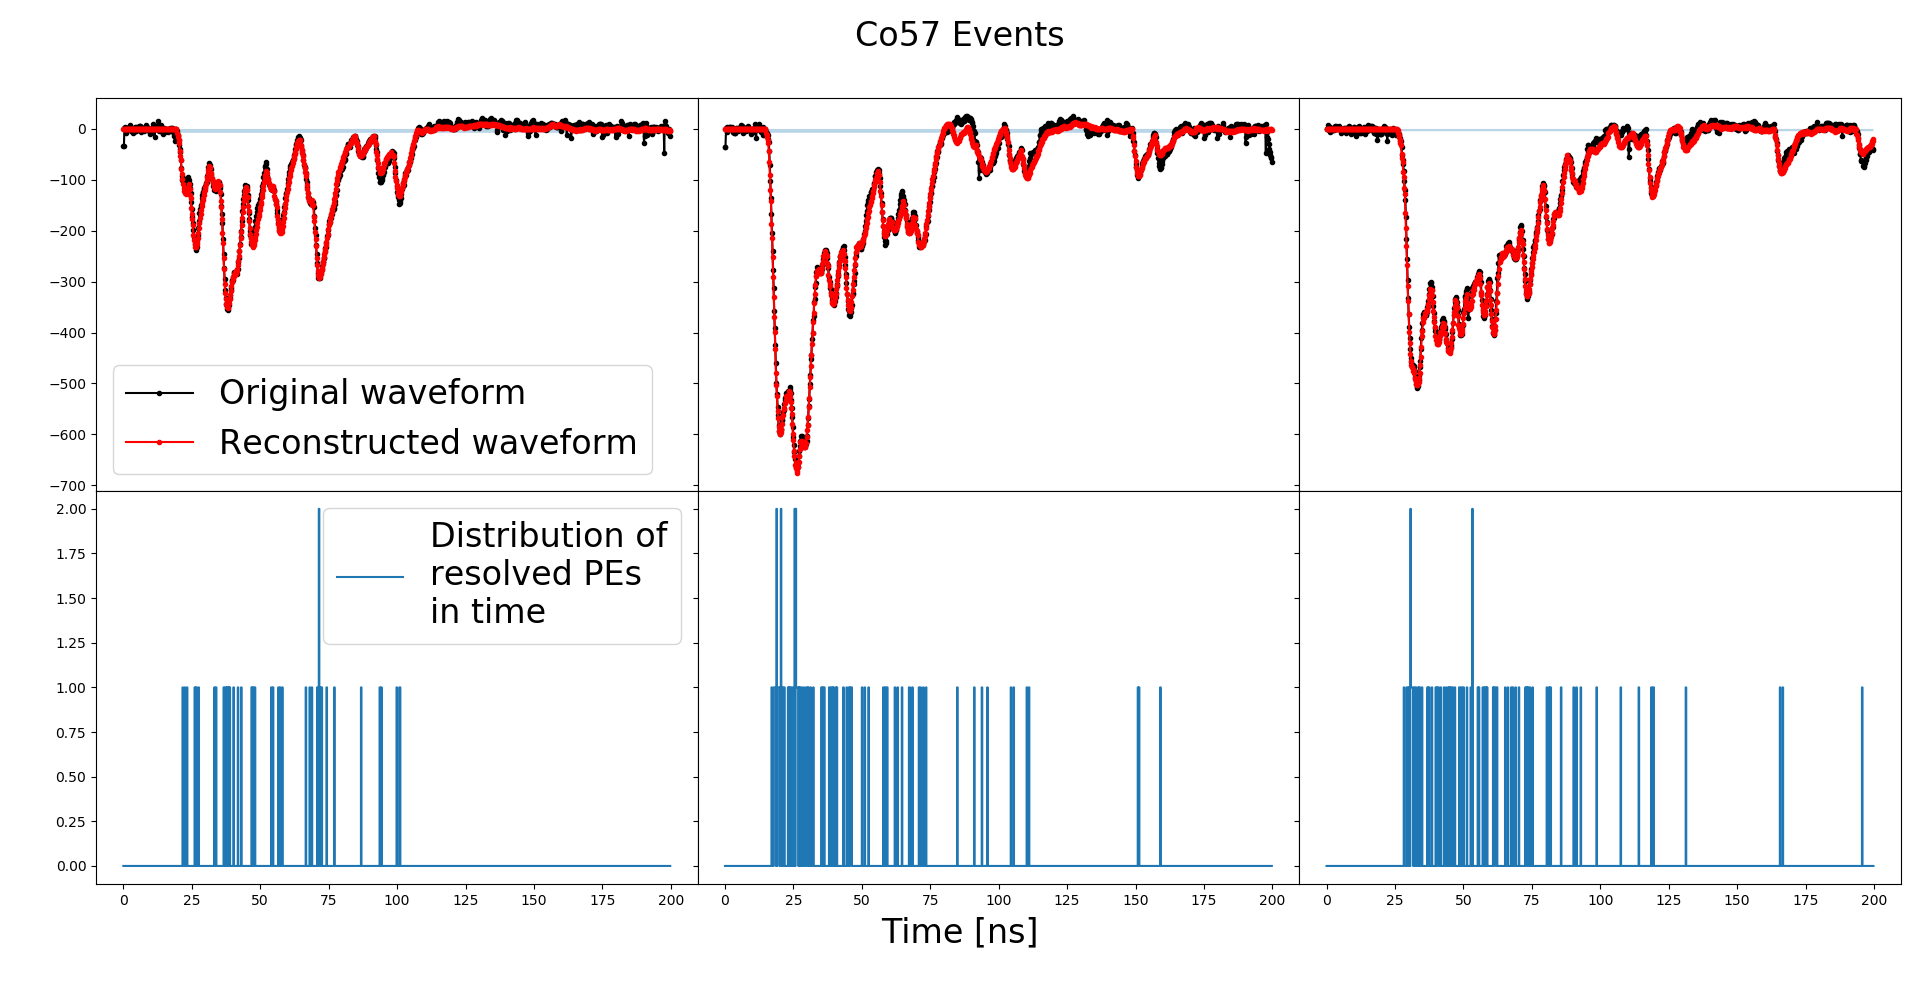
\includegraphics[width=1\textwidth]{recons.png}
\end{figure}
\end{frame}

\begin{frame}{SPE Calibration}

\end{frame}

\begin{frame}{Event Reconstruction Algorithm}

\end{frame}

\begin{frame}{Data Selection - PMT flashing}
After reconstruction some quality cuts are made ($\chi^2$, blw and first PE). Then also PMT flashing events are cut out. This events are characterized by the amount of the PEs in the first 10 ns of the event relative to full amount of the PEs ($\omega$). Events with $\omega>0.5$ are cut out. This events assumed to be generated by the PMTs because such events were found also when there were no sphere in the setup (both Co and Cs datasets gives $0.15$~Hz of PMT fleshing). 
\begin{figure}[h]
    \centering
    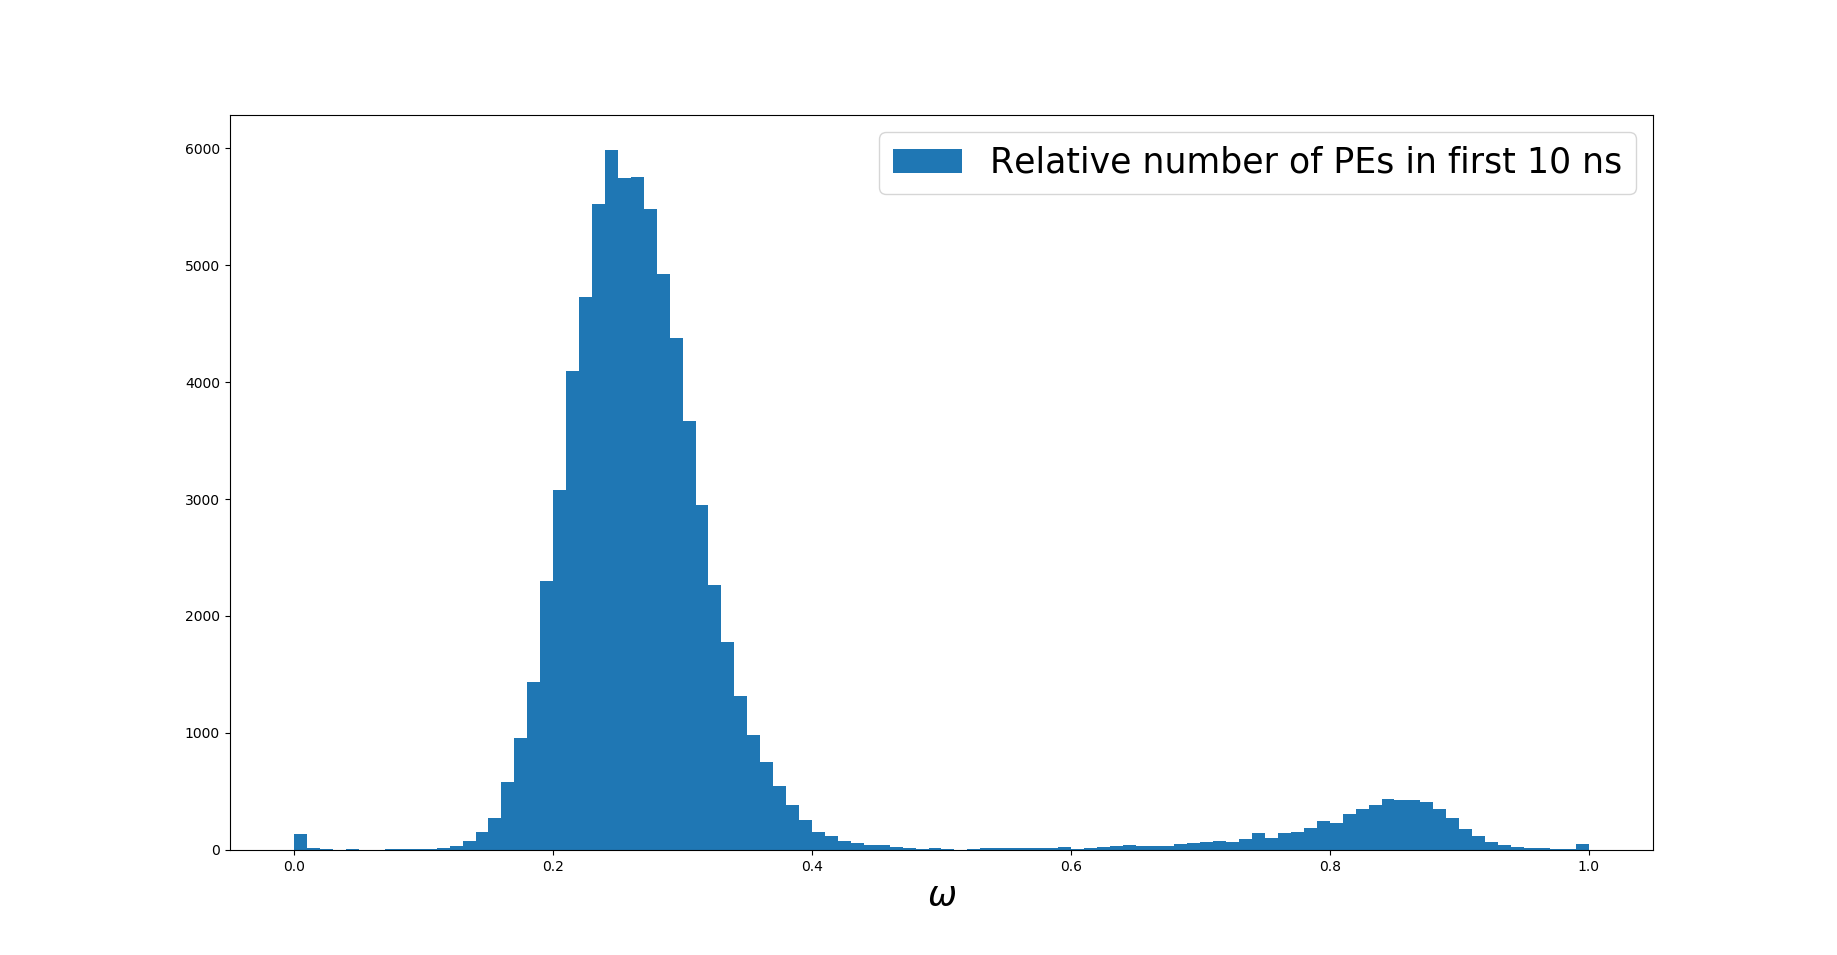
\includegraphics[width=0.75\textwidth]{w.png}
\end{figure}
\end{frame}

\begin{frame}{Data Selection - ?}
\begin{figure}
\subfloat{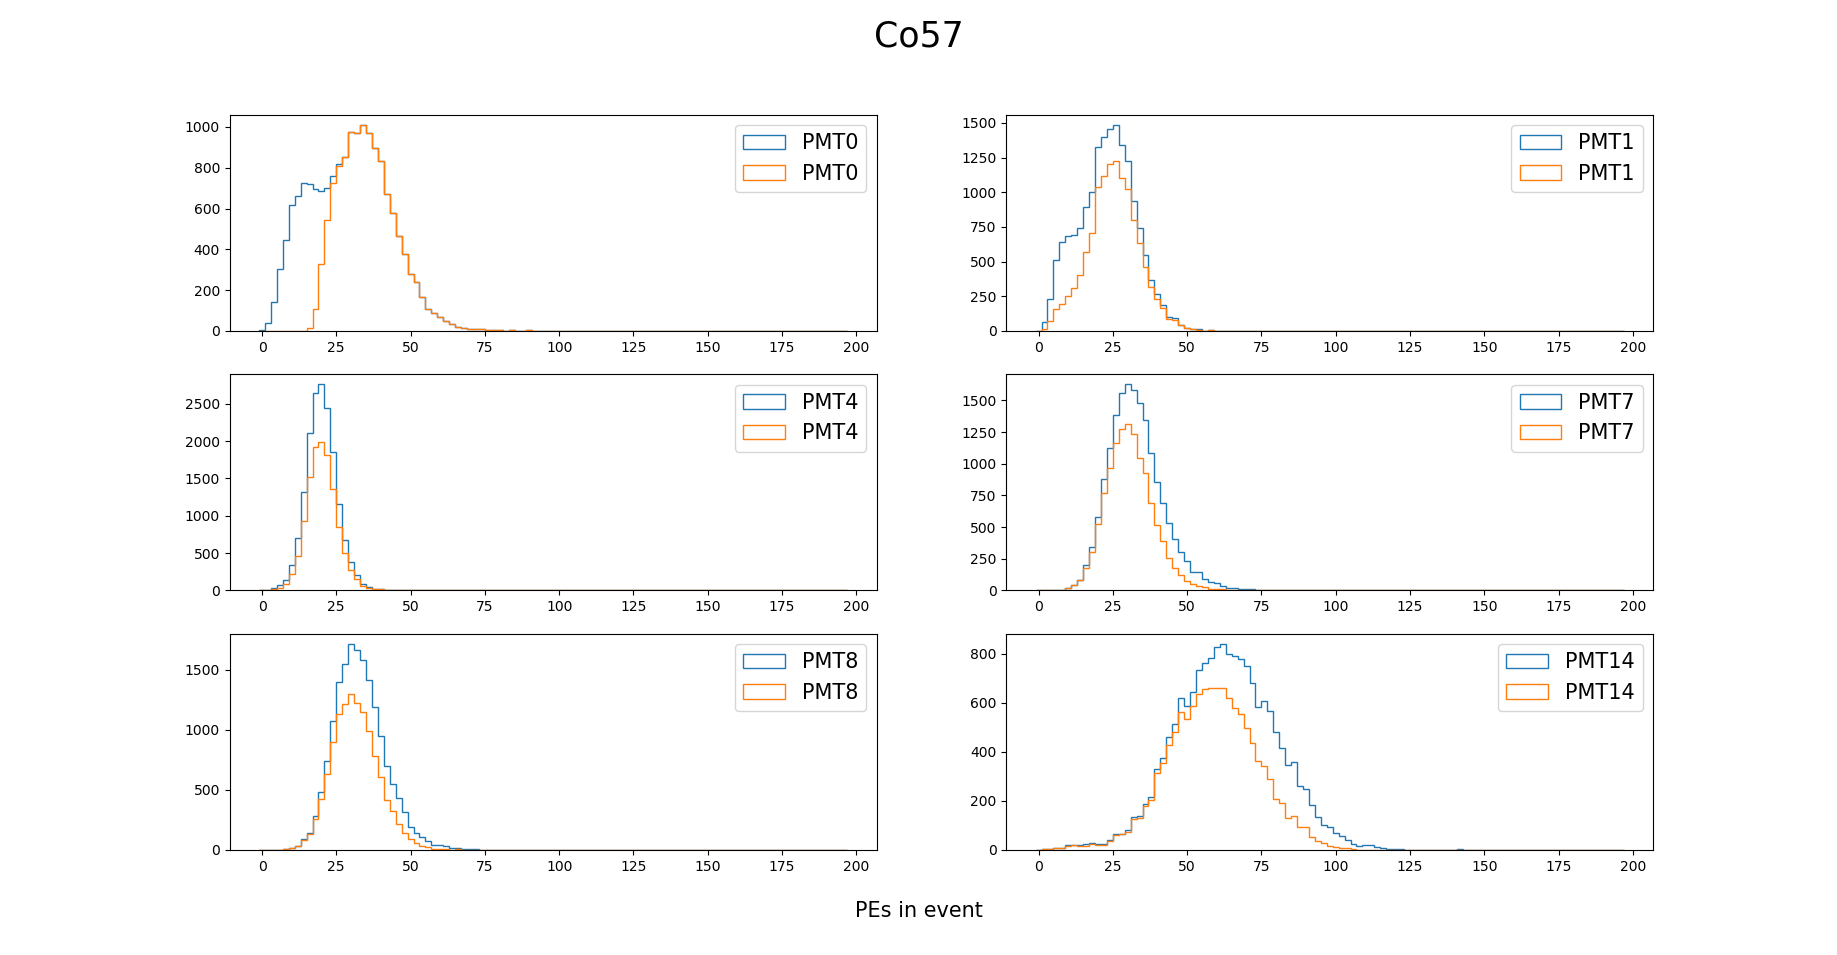
\includegraphics[width=0.45\textwidth]{UpDown.png}}\qquad
  \subfloat{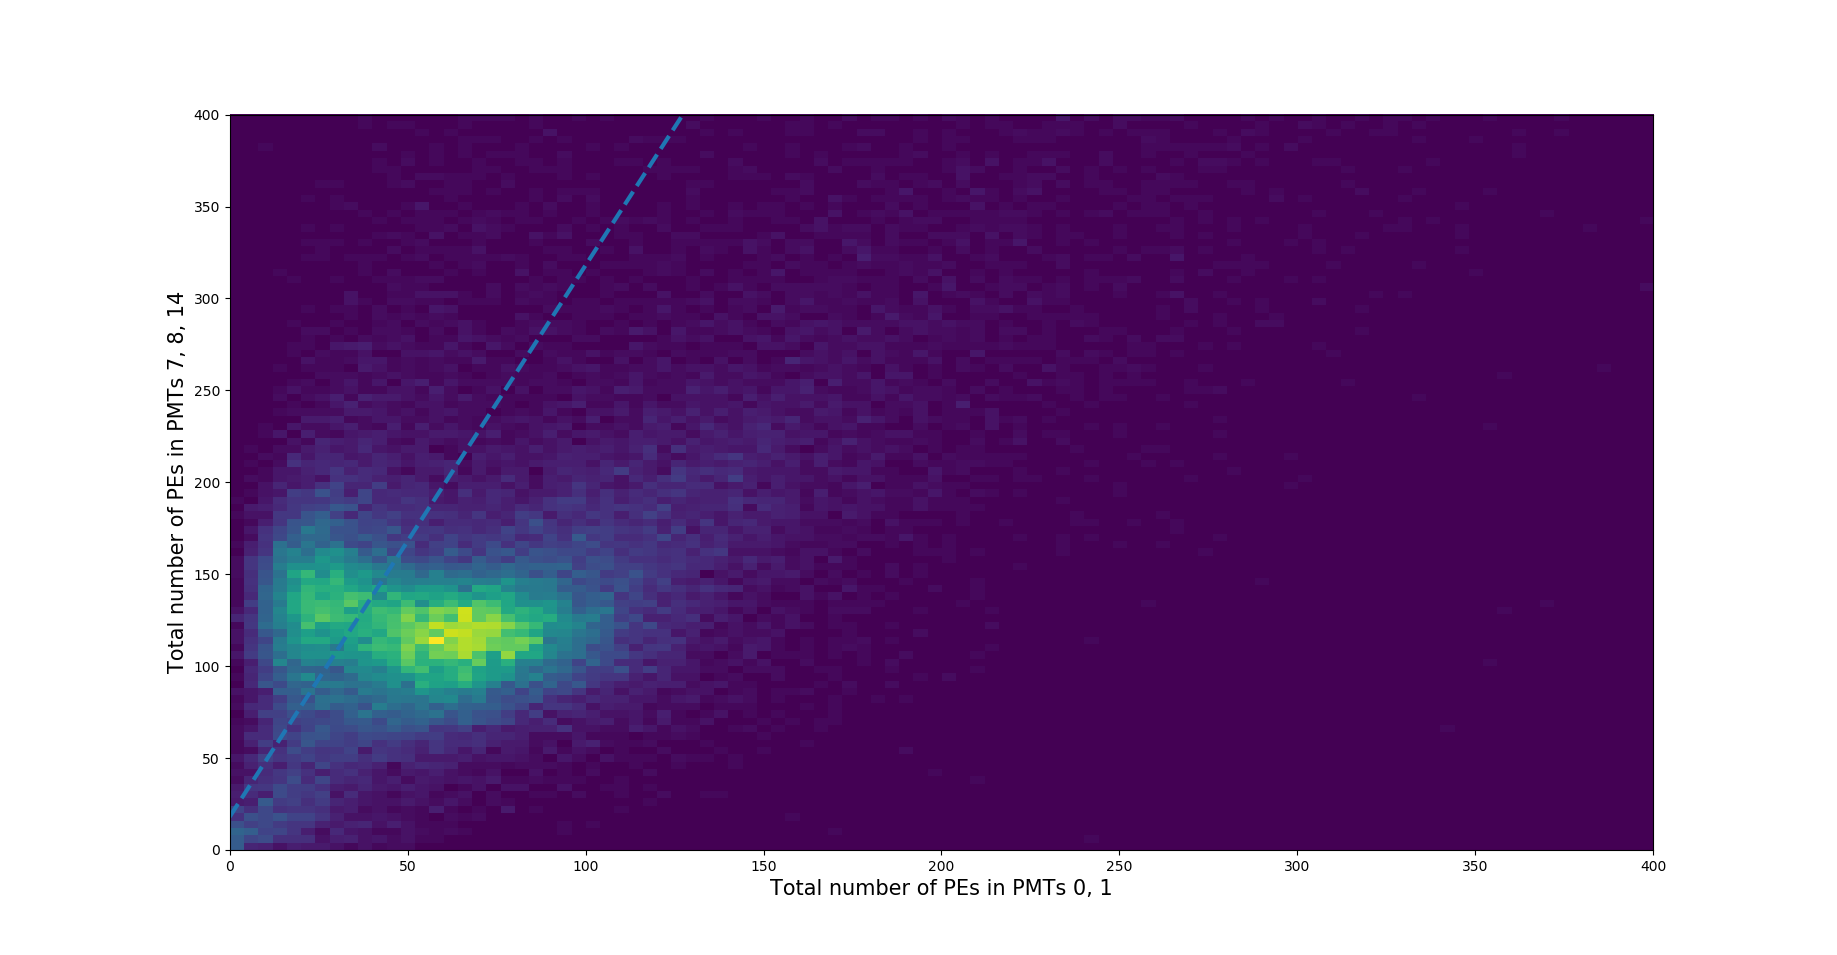
\includegraphics[width=0.45\textwidth]{UpDown2D.png}}
\end{figure}
There is a weird feature in the spectra that I still cant understand. There is a subpopulation of events in which PMTs 0,1 sees less PEs then expected, and PMTs 7,8,14 sees more then expected. I cut these events based on the ratio between the total number PEs in the first PMT group and the second group. 
\end{frame}

\begin{frame}{Data Selection - Spectrum}
\begin{figure}
Finally, only events around the full absorption peak are chosen
\subfloat[$^{57}$Co]{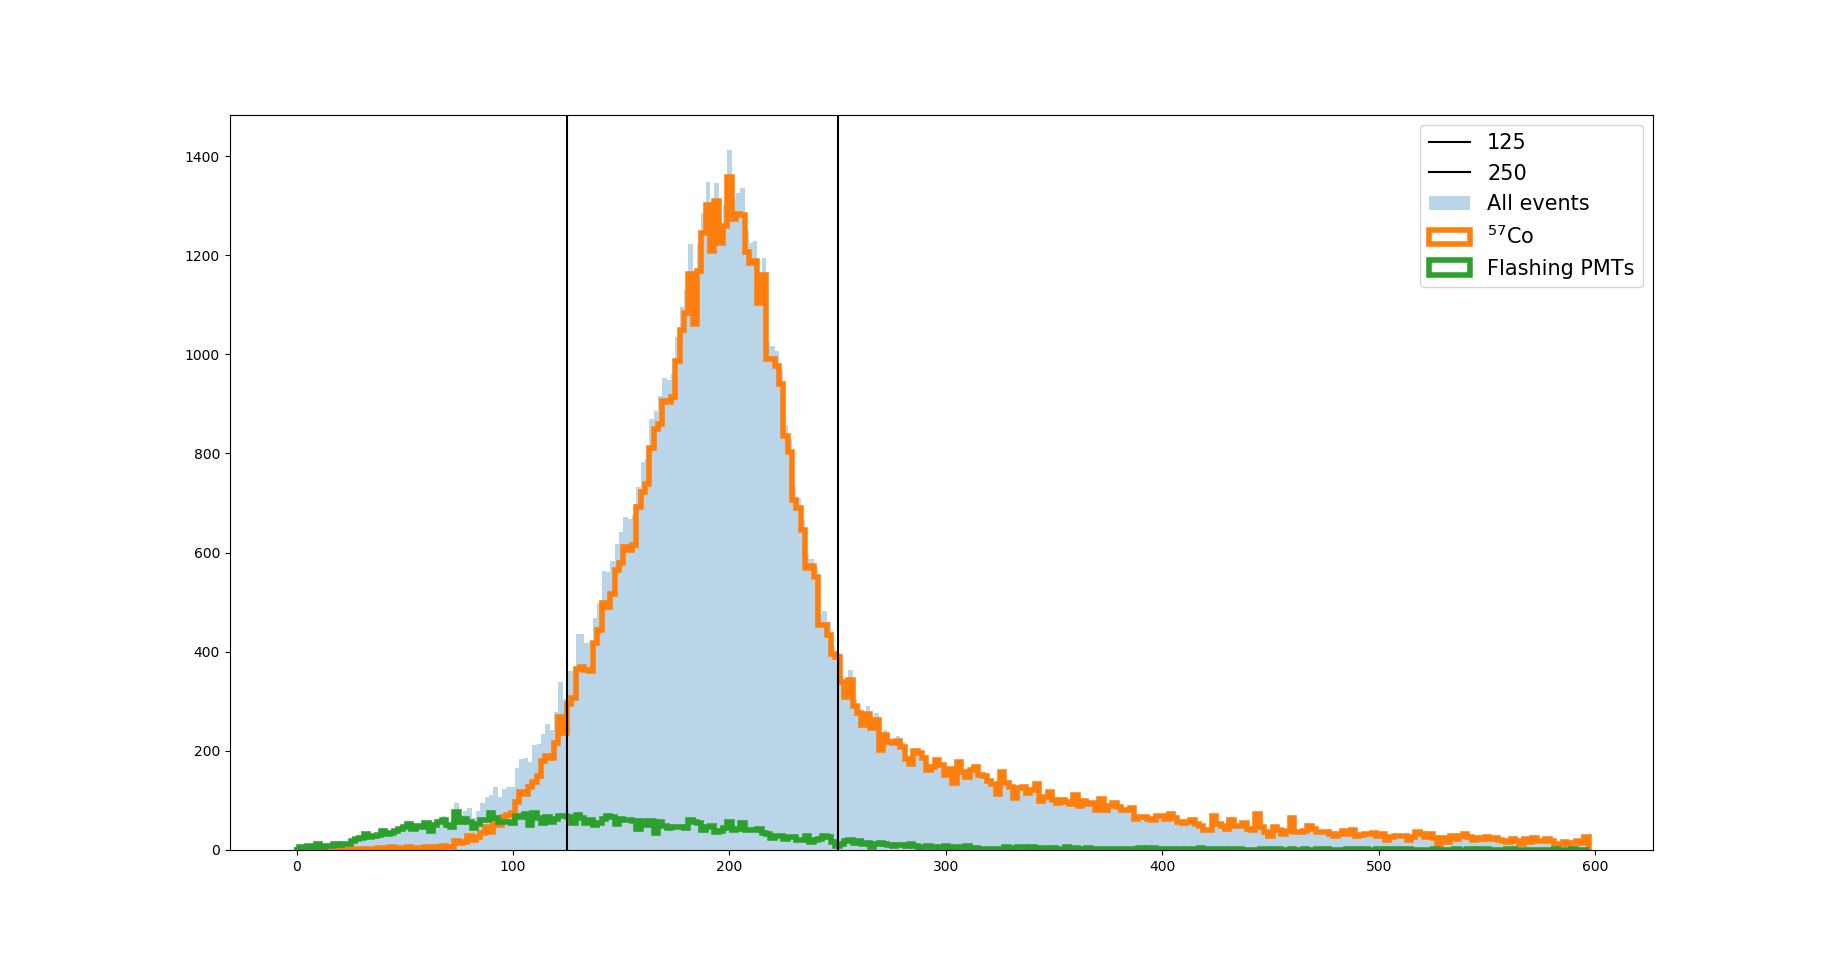
\includegraphics[width=0.5\textwidth]{Co57.png}}\qquad
  \subfloat[$^{137}$Cs]{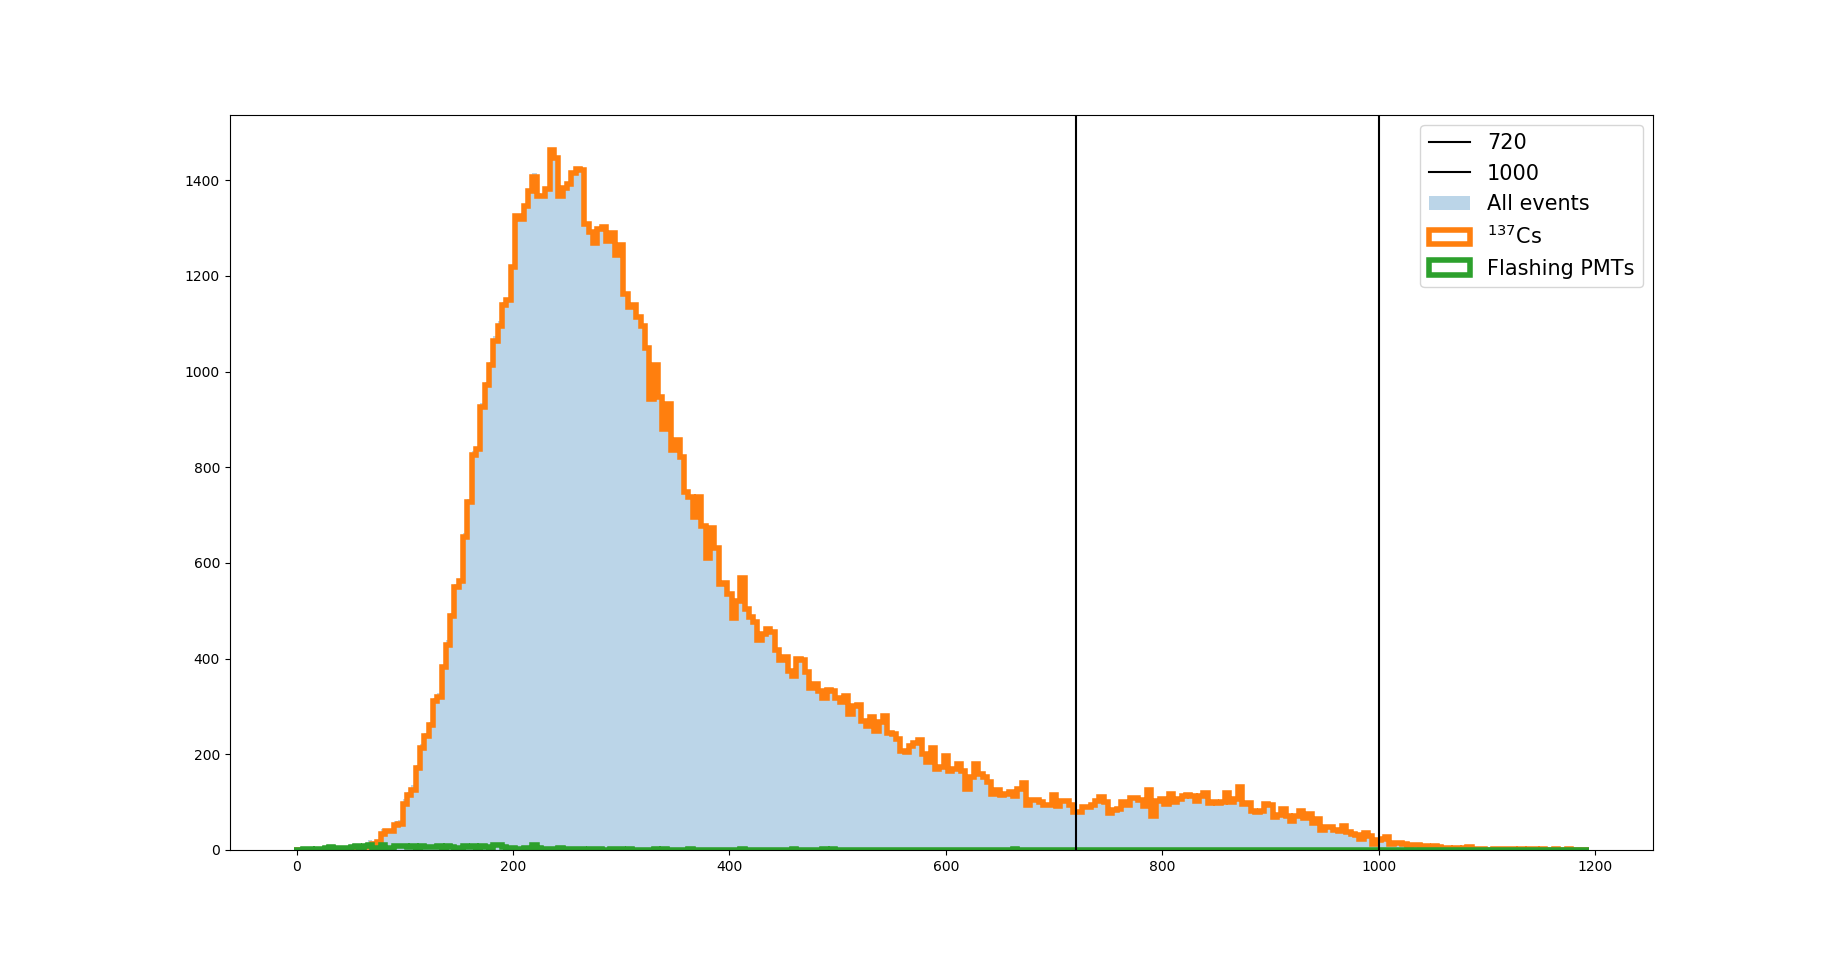
\includegraphics[width=0.5\textwidth]{Cs137.png}}
\end{figure}
\end{frame}

\begin{frame}{Average Temporal Structure}
\begin{figure}[h]
    \centering
    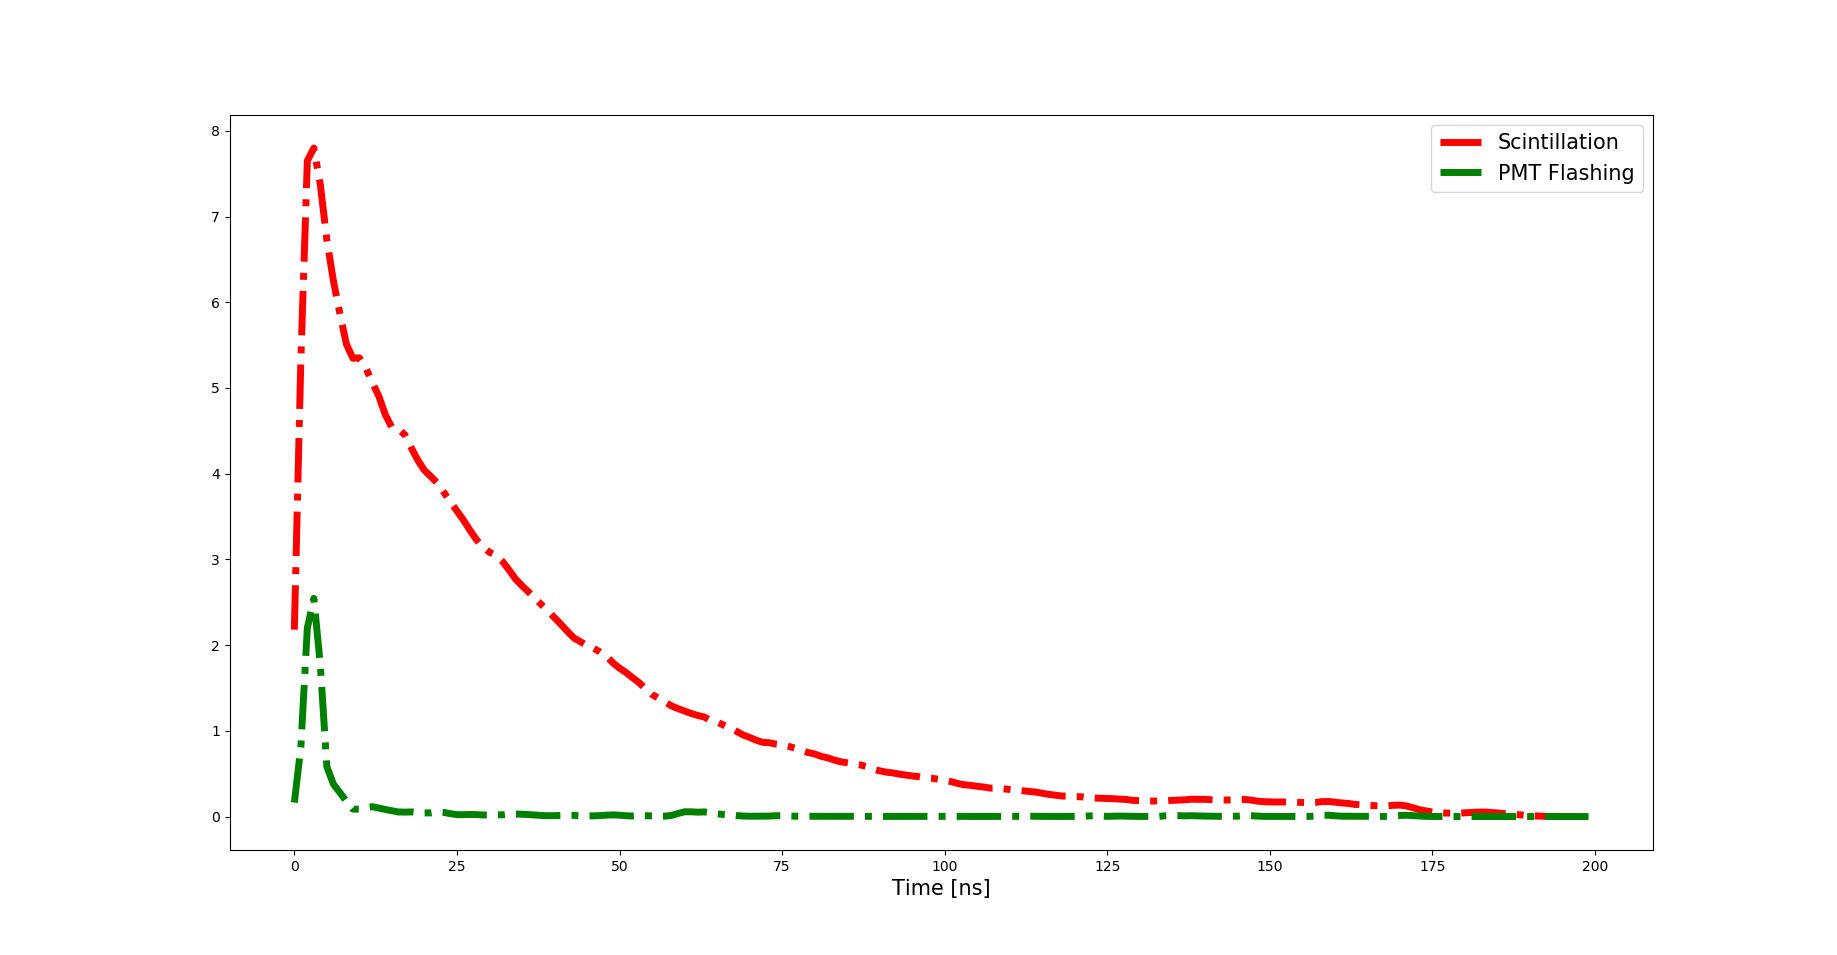
\includegraphics[width=1\textwidth]{temp.png}
\end{figure}
\end{frame}

\begin{frame}{The Dataset $D_{nia}$ and the Model $H_{nia}$}
For each measurement a 3D table ($D_{nia}$) is build. It holds the number of events in which $n$ PEs were resolved at time $i$ (after the first PE in the events) in PMT $a$.\\

\begin{equation}
\frac{1}{N_{\text{events}}}\sum_{n,a}nD_{nia}
\end{equation}
is the average temporal structure shown above.\\
\quad\\
We want to use a scintillation model to build a similar 3D table ($H_{nia}$) and fit it to the dataset.
\end{frame}


\begin{frame}{Scintillation Model}
The probability that $\nu$ PEs were resolved at time window $[t_i-dt/2, t_i+dt/2]$ by PMT $a$, given that $n$ photons were created at the event is
\begin{equation}
B_{\nu ian}=\text{Binom}(\nu|n,d\Omega_aQ_adtY_{i})
\end{equation}
where $d\Omega_a$ and $Q_a$ are the solid angle and the light detection efficiency of PMT $a$ and $Y_i$ is the probability to emit a photon at time window $i$.

\blfootnote{Light detection efficiency is all the mechanisms which generates $m$ PEs from $n>m$ photons that hit the face of the PMT. This includes quantum efficiency, collection efficiency, double PE probability and more}
\end{frame}

\begin{frame}{Scintillation Model - Time Smearing}
Each PMT has its temporal resolution ($\sigma_a$) and a delay ($T_a$).
This means that a PE that was created at time $i$ has a probability to be resolved at time $j$. This probability is
\begin{equation}
P_{ij}=\frac{dt}{\sqrt{2\pi}\sigma_a}e^{-(t_j-t_i-T_a)^2/2\sigma_a^2}
\end{equation}
Thus
\begin{equation}
Y_i\rightarrow Y_{ja}=\int_0^{\infty}Y_{t_i}\frac{dt}{\sqrt{2\pi}\sigma_a}e^{-(t_j-t_i-T_a)^2/2\sigma_a^2}
\end{equation}

\end{frame}

\begin{frame}{Scintillation Model - Alignment by the First PE}
The probability that PMT $a$ will resolve $\nu>0$ PEs at the same time window as the first PE in the event (this goes to $H_{\nu0a}$), given that $n$ photons were created at the event is
\begin{equation}
P_{\nu0a}=\sum_j\prod_{k<j}\prod_bB_{0kbn}B_{\nu jan}.
\end{equation}
To get the model for the 3D array ($H_{\nu ia}$) the number of the photons per event needs to be averaged
\begin{equation}
H_{\nu0a}=\sum_{j,n}\prod_{k<j}\prod_bB_{0kbn}B_{\nu jan}\text{Poisson}(n|N)
\end{equation}
were $N$ is the average number of photons created in the interaction.
\end{frame}

\begin{frame}{Scintillation Model - Alignment by the First PE}
The probability that PMT $a$ will resolve $0$ PEs at the same time window as the first PE in the event (this goes to $H_{00a}$), given that $n$ photons were created at the event is
\begin{equation}
P_{00a}=\sum_j\prod_{k<j}\prod_bB_{0kbn}(1-\prod_{c\neq a}B_{0jcn})B_{0jan}.
\end{equation}
So
\begin{equation}
H_{00a}=\sum_{j,n}\prod_{k<j}\prod_bB_{0kbn}(1-\prod_{c\neq a}B_{0jcn})B_{0jan}\text{Poisson}(n|N)
\end{equation}
\end{frame}


\begin{frame}{Scintillation Model - Alignment by the First PE}
The probability that PMT $a$ will resolve $\nu$ PEs at time window $i$ after the first PE in the event (this goes to $H_{\nu ia}$), given that $n$ photons were created at the event is
\begin{equation}
P_{\nu ia}=\sum_j\prod_{k<j}\prod_bB_{0kbn}(1-\prod_bB_{0jbn})B_{\nu j+ian}.
\end{equation}
So
\begin{equation}
H_{\nu0a}=\sum_j\prod_{k<j}\prod_bB_{0kbn}(1-\prod_bB_{0jbn})B_{\nu j+ian}\text{Poisson}(n|N)
\end{equation}
\end{frame}

\begin{frame}{Temporal Scintillation Model - $Y(t)$}
Primary scintillation (singlet ($\tau_1$) and triplet ($\tau_3$)):
\begin{equation}
Y_P(t)=\frac{F}{\tau_1}e^{-t/\tau_1}+\frac{1-F}{\tau_3}e^{-t/\tau_3}
\end{equation}
Secondary scintillation (recombination):
\begin{equation}
Y_R(t)=\int_0^t\left(\frac{F}{\tau_1}e^{-(t-\tilde{t})/\tau_1}+\frac{1-F}{\tau_3}e^{-(t-\tilde{t})/\tau_3}\right)P_R(\tilde{t})d\tilde{t}
\end{equation}
where $P_R(t)$ is the probability for recombination at time $t$ after the beginning of the event.
\blfootnote{We assume here that the singlet-triplet branching at the secondary scintillation is the same as in the primary.}
\end{frame}

\begin{frame}{Recombination}
It is customary to model the recombination as
\begin{equation}
\frac{dN_+}{dt}=-\alpha N_+N_-
\end{equation}
with the initial conditions of
\begin{equation}
N_+(t=0)=RN \quad N_-(t=0)=(\eta-1)RN
\end{equation}

$\eta$ is the fraction of ionized electrons which escapes recombination and $R$ is the fraction of the energy deposition which goes to ionization and not recombine immediately with its parent ion (geminate/Onsager recombination).  
\end{frame}

\begin{frame}{Combined Scintillation Model}
\begin{equation}
Y(t)=(1-R)Y_P(t)+(1-\eta)RY_R(t)
\end{equation}
\end{frame}

\begin{frame}{Fit - Temporal Distribution per PMT - $^{57}$Co}
\begin{figure}[h]
\centering
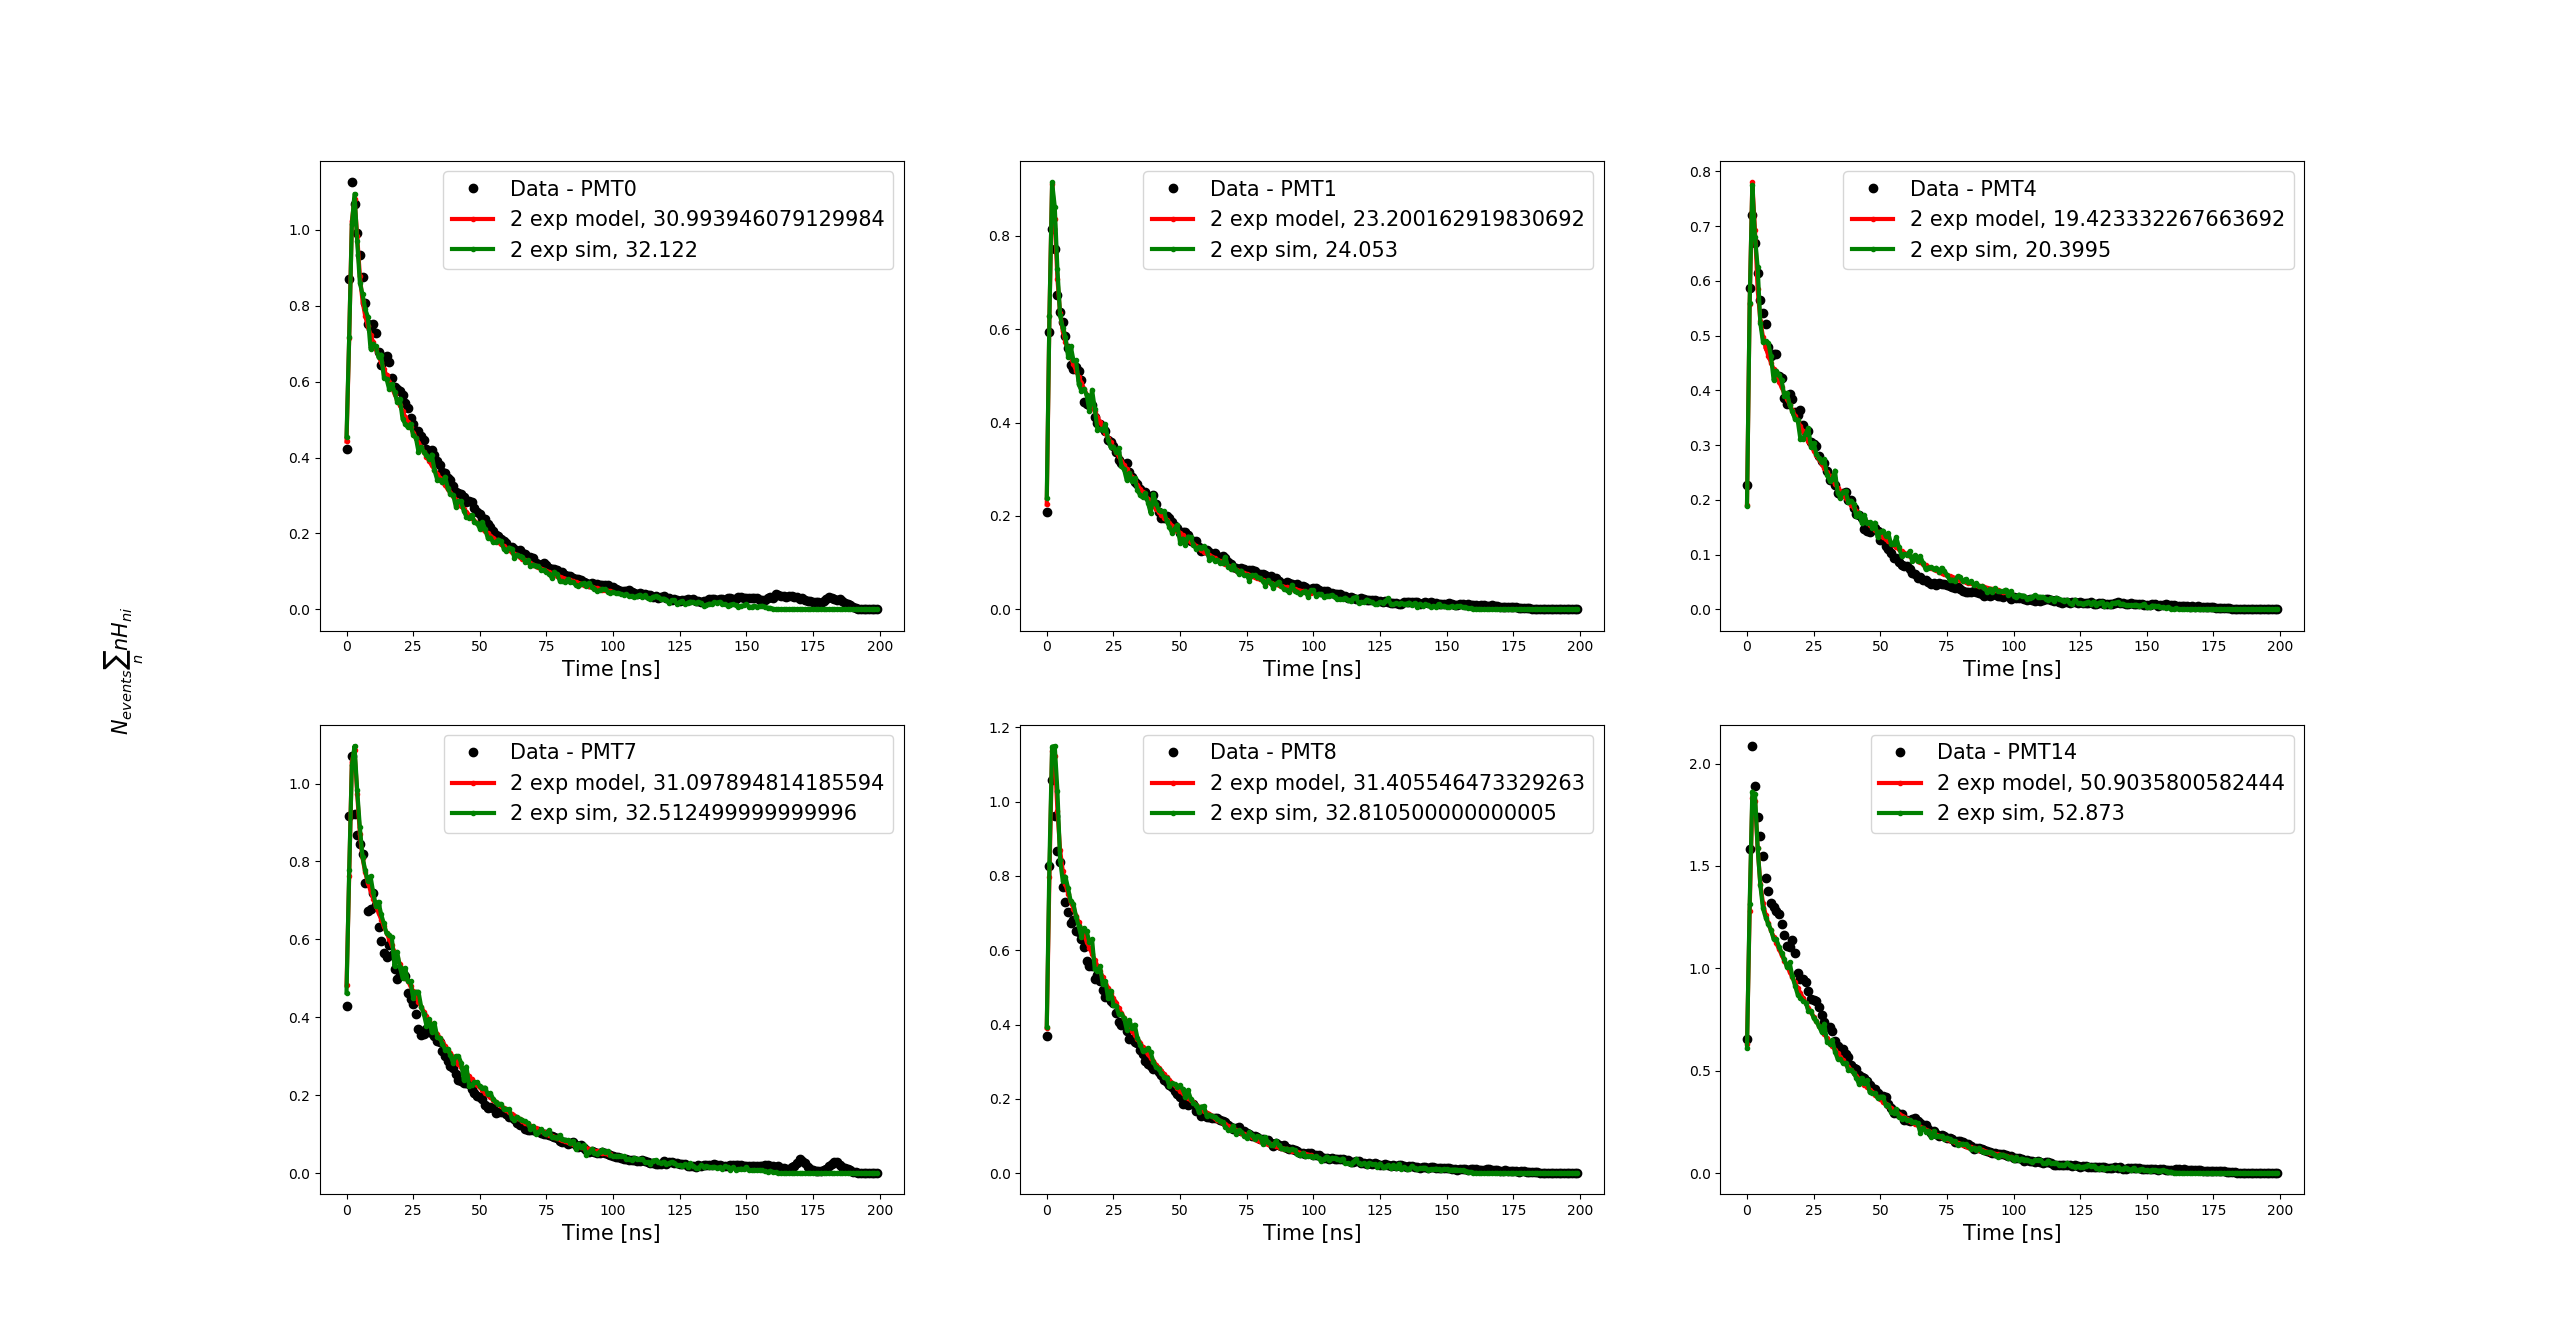
\includegraphics[width=1\textwidth]{Co576PMTs.png}
\end{figure}
\end{frame}

\begin{frame}{Fit - Temporal Distribution per PMT - $^{137}$Cs}
\begin{figure}[h]
\centering
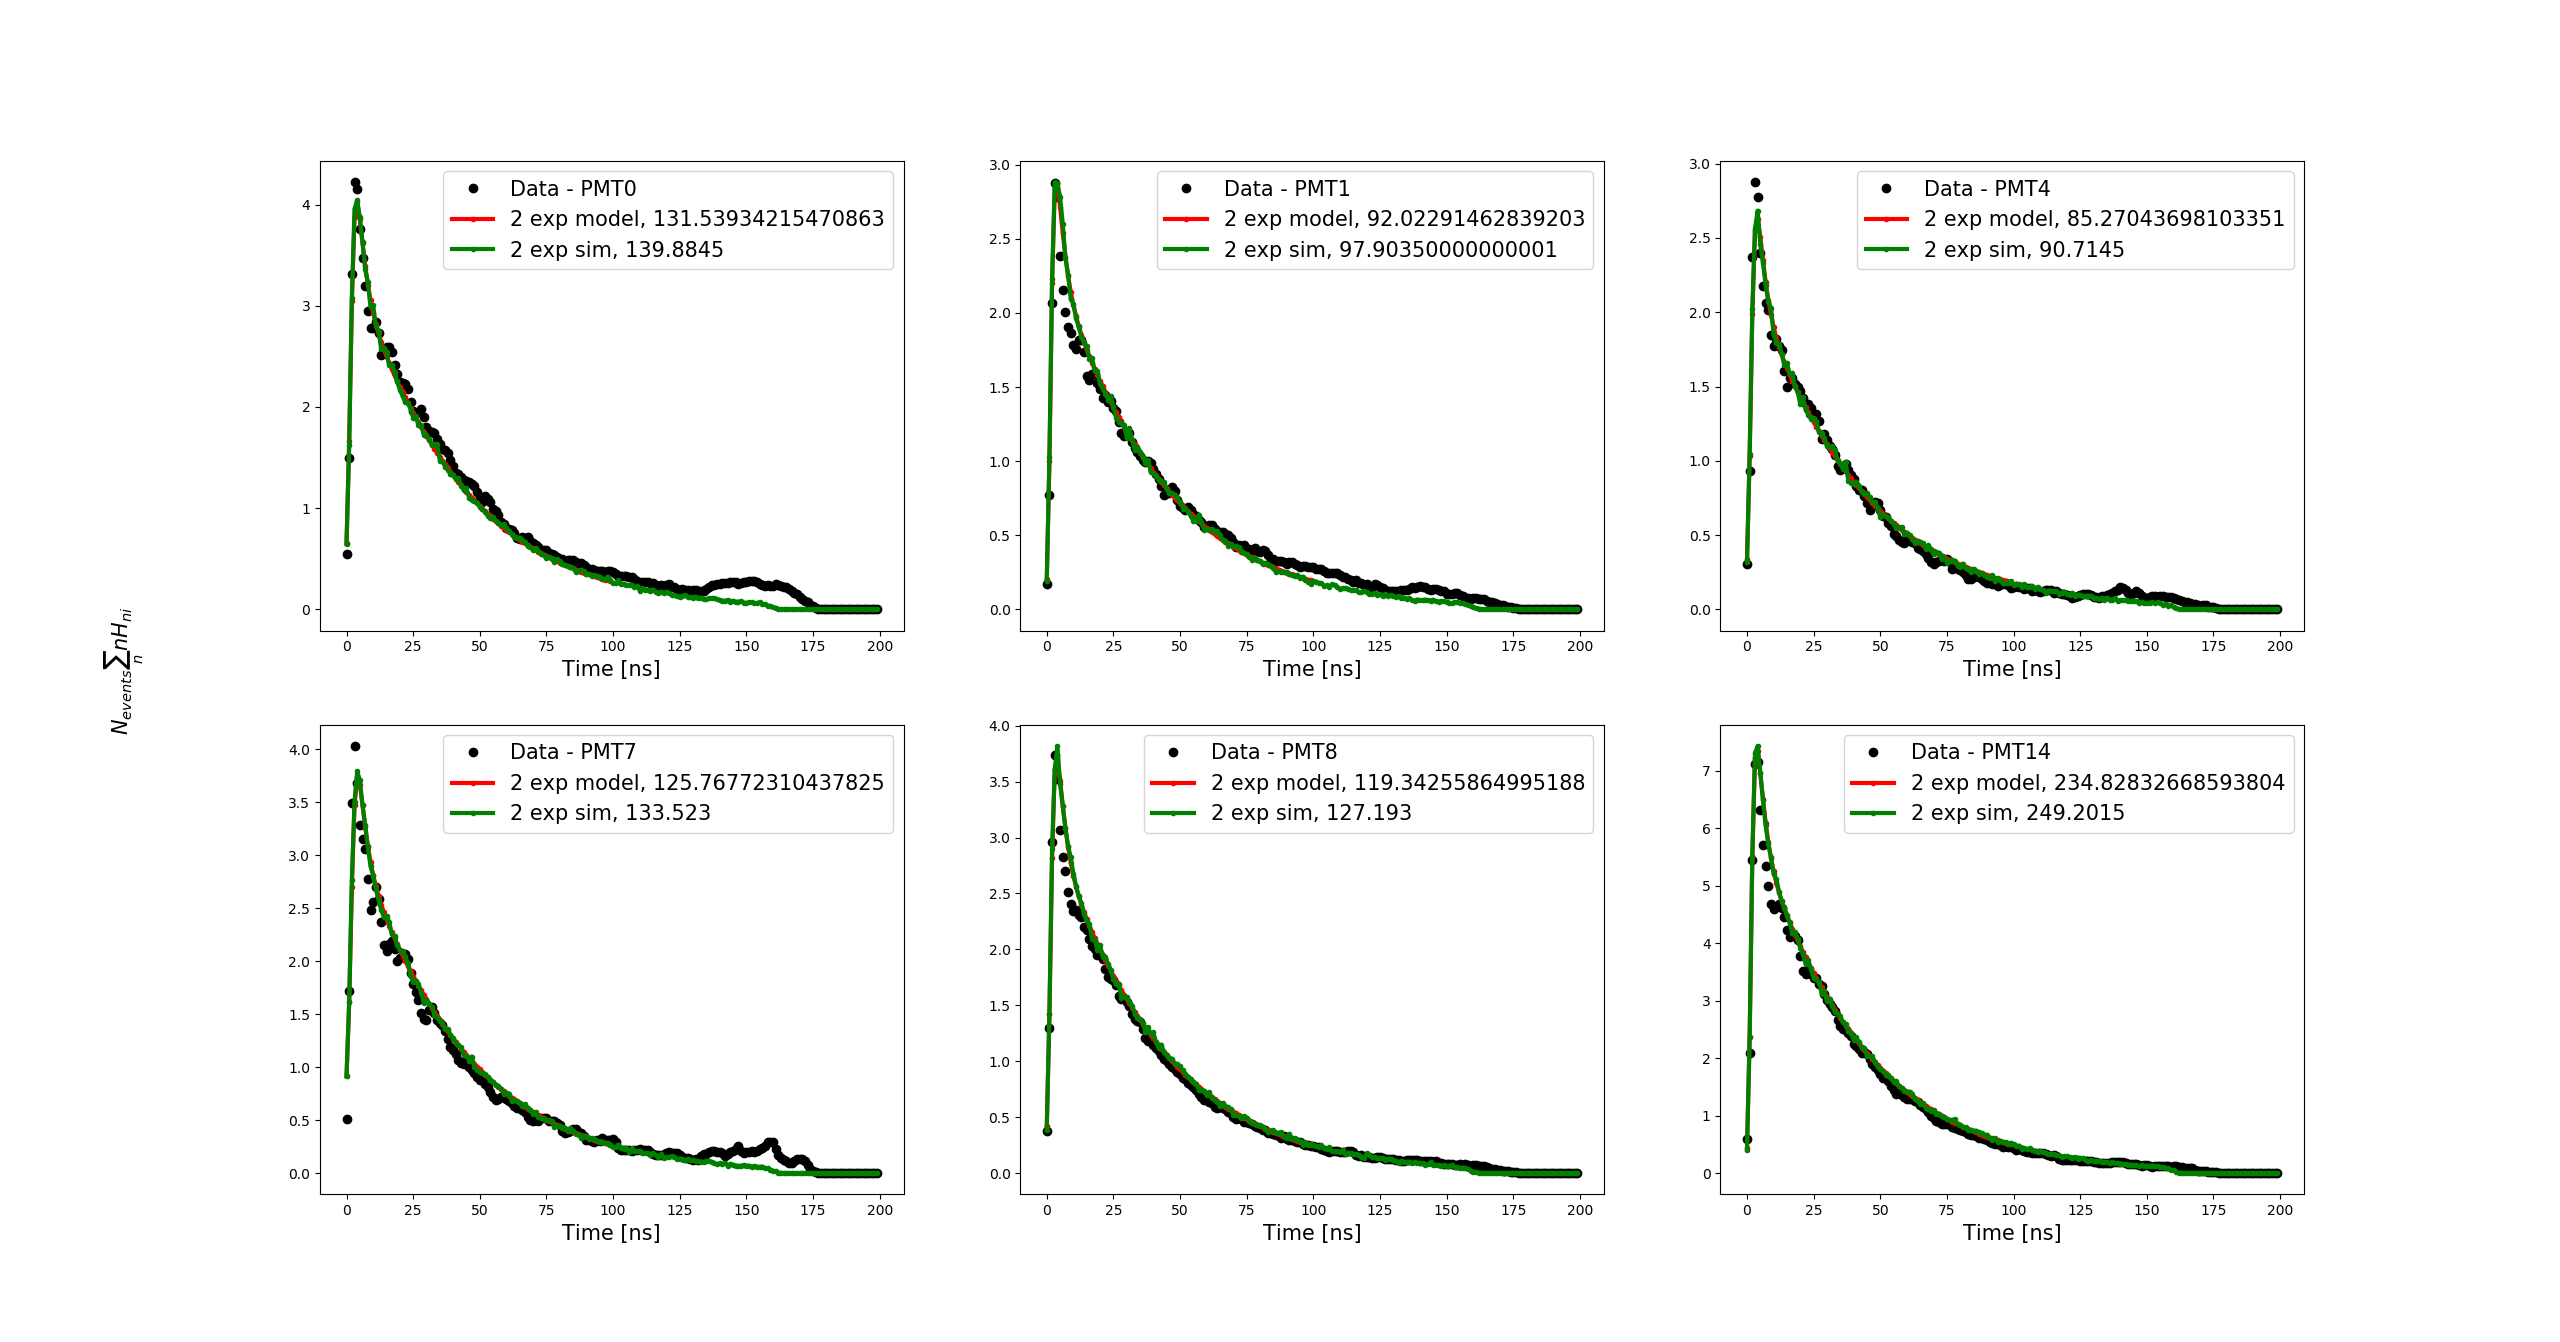
\includegraphics[width=1\textwidth]{Cs1376PMTs.png}
\end{figure}
\end{frame}

\begin{frame}{Fit - Spectra per PMT - $^{57}$Co}
\begin{figure}[h]
\centering
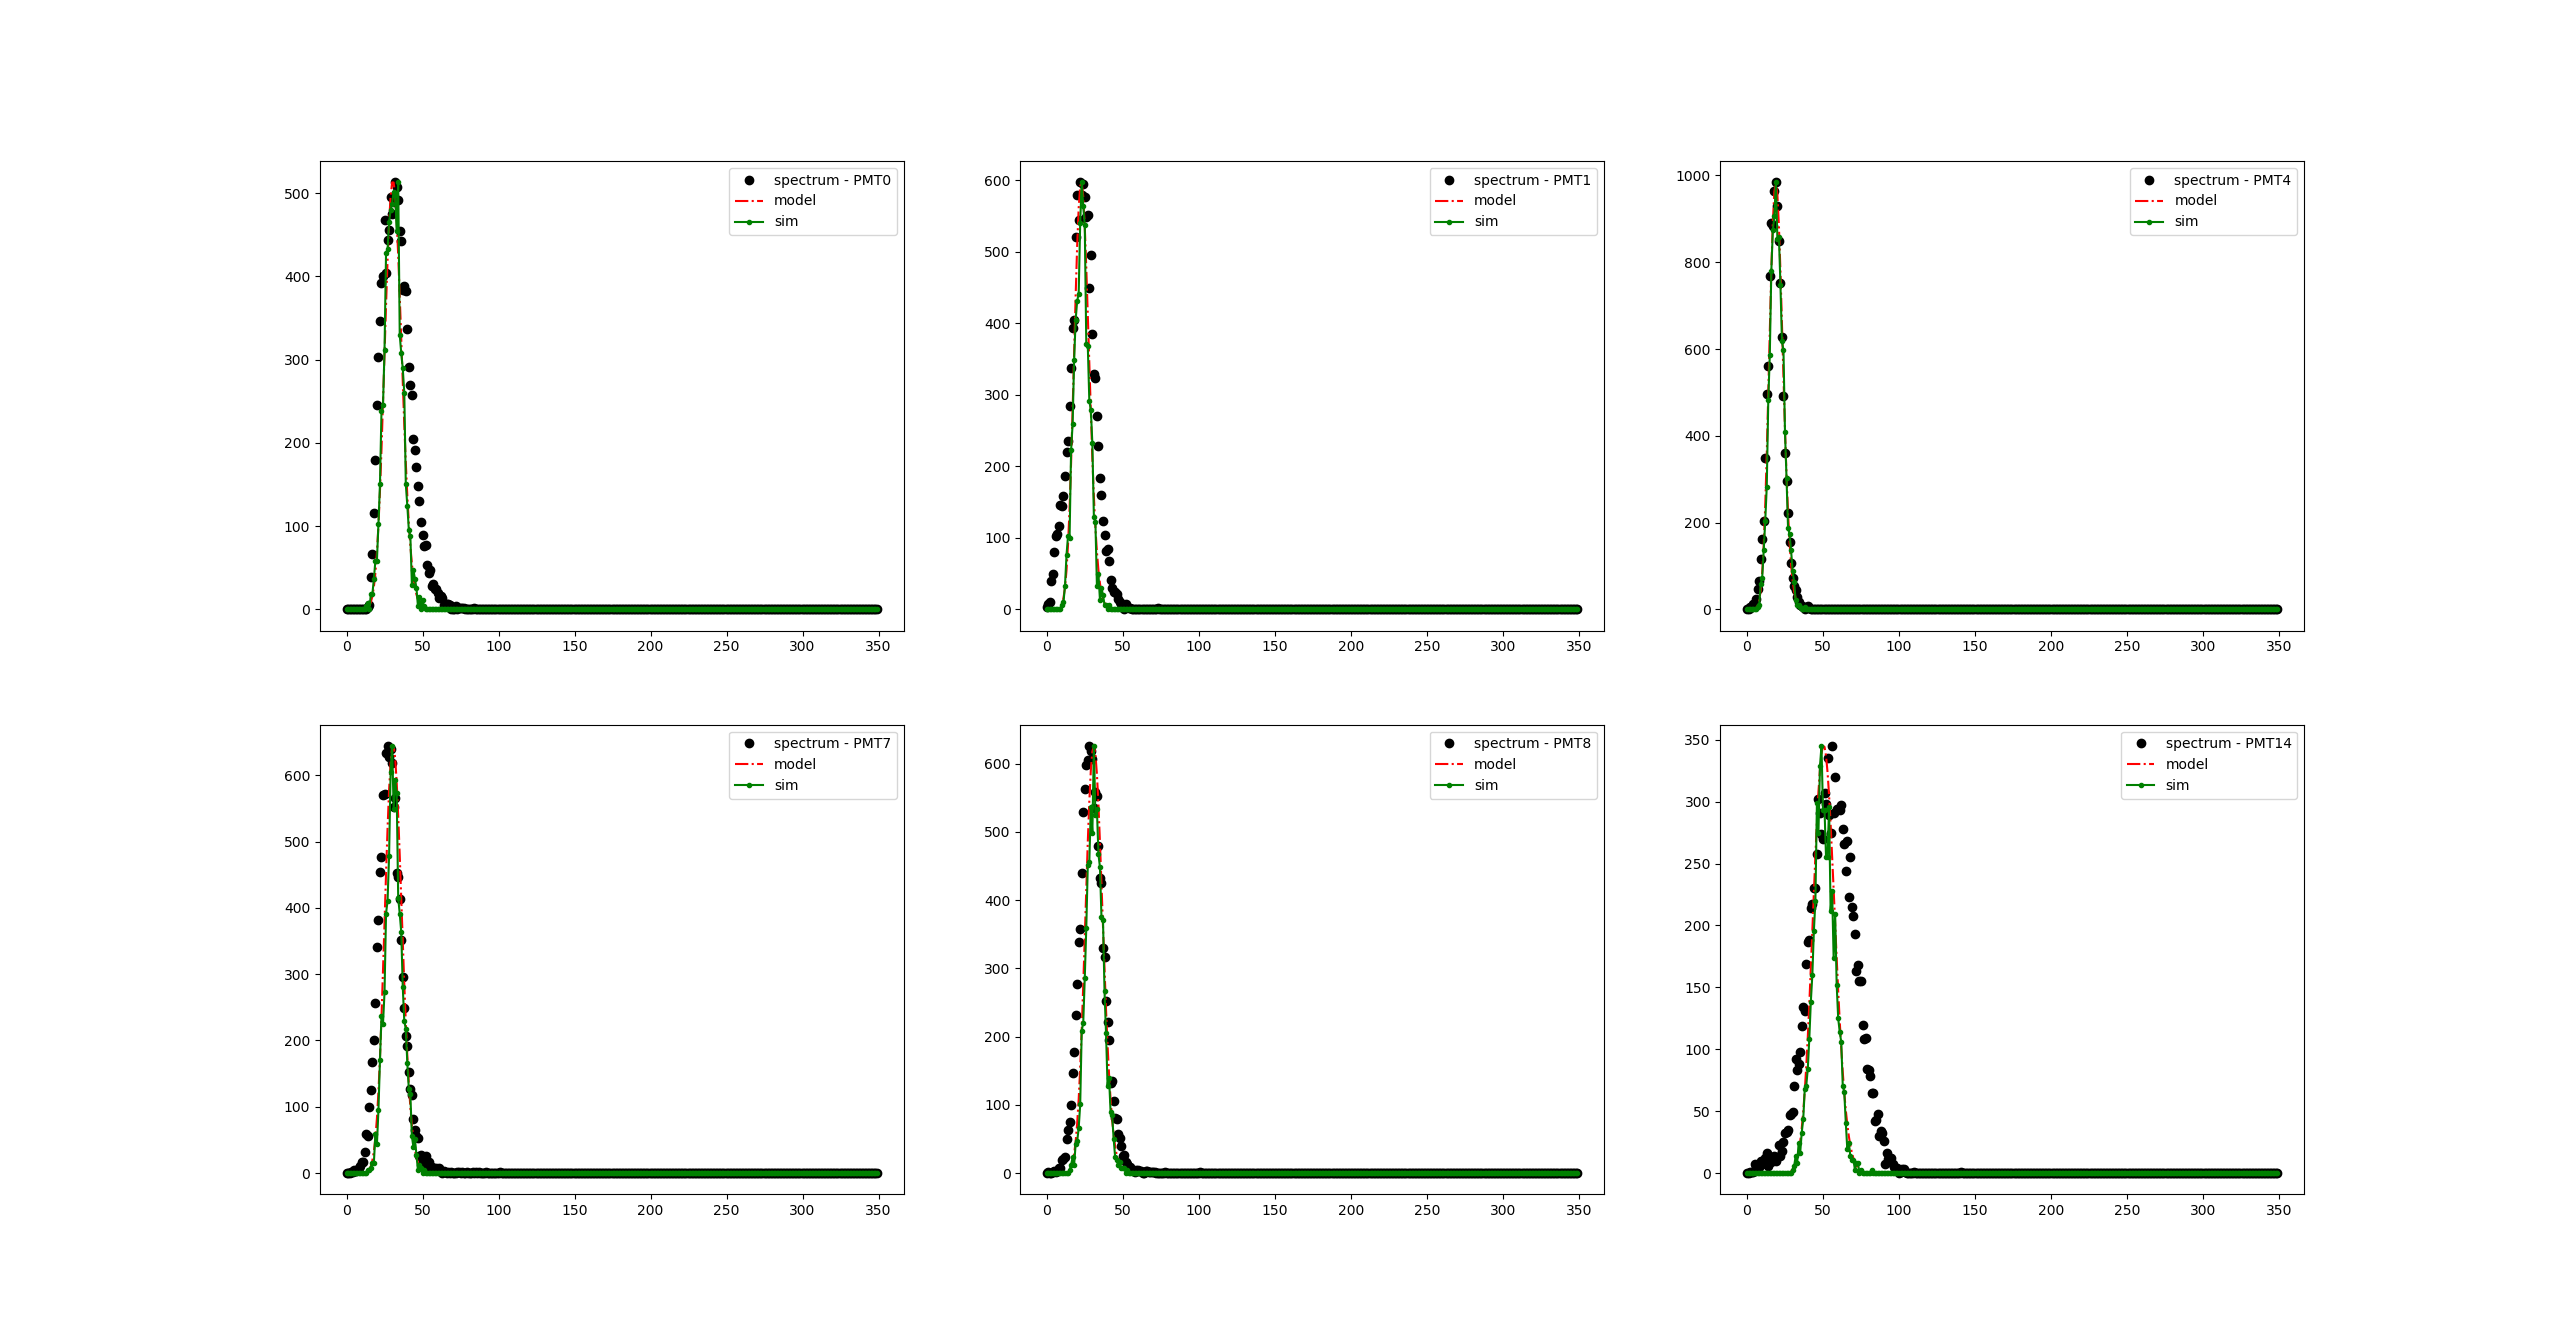
\includegraphics[width=1\textwidth]{Co57Spec.png}
\end{figure}
\end{frame}

\begin{frame}{Fit - Spectra per PMT - $^{137}$Cs}
\begin{figure}[h]
\centering
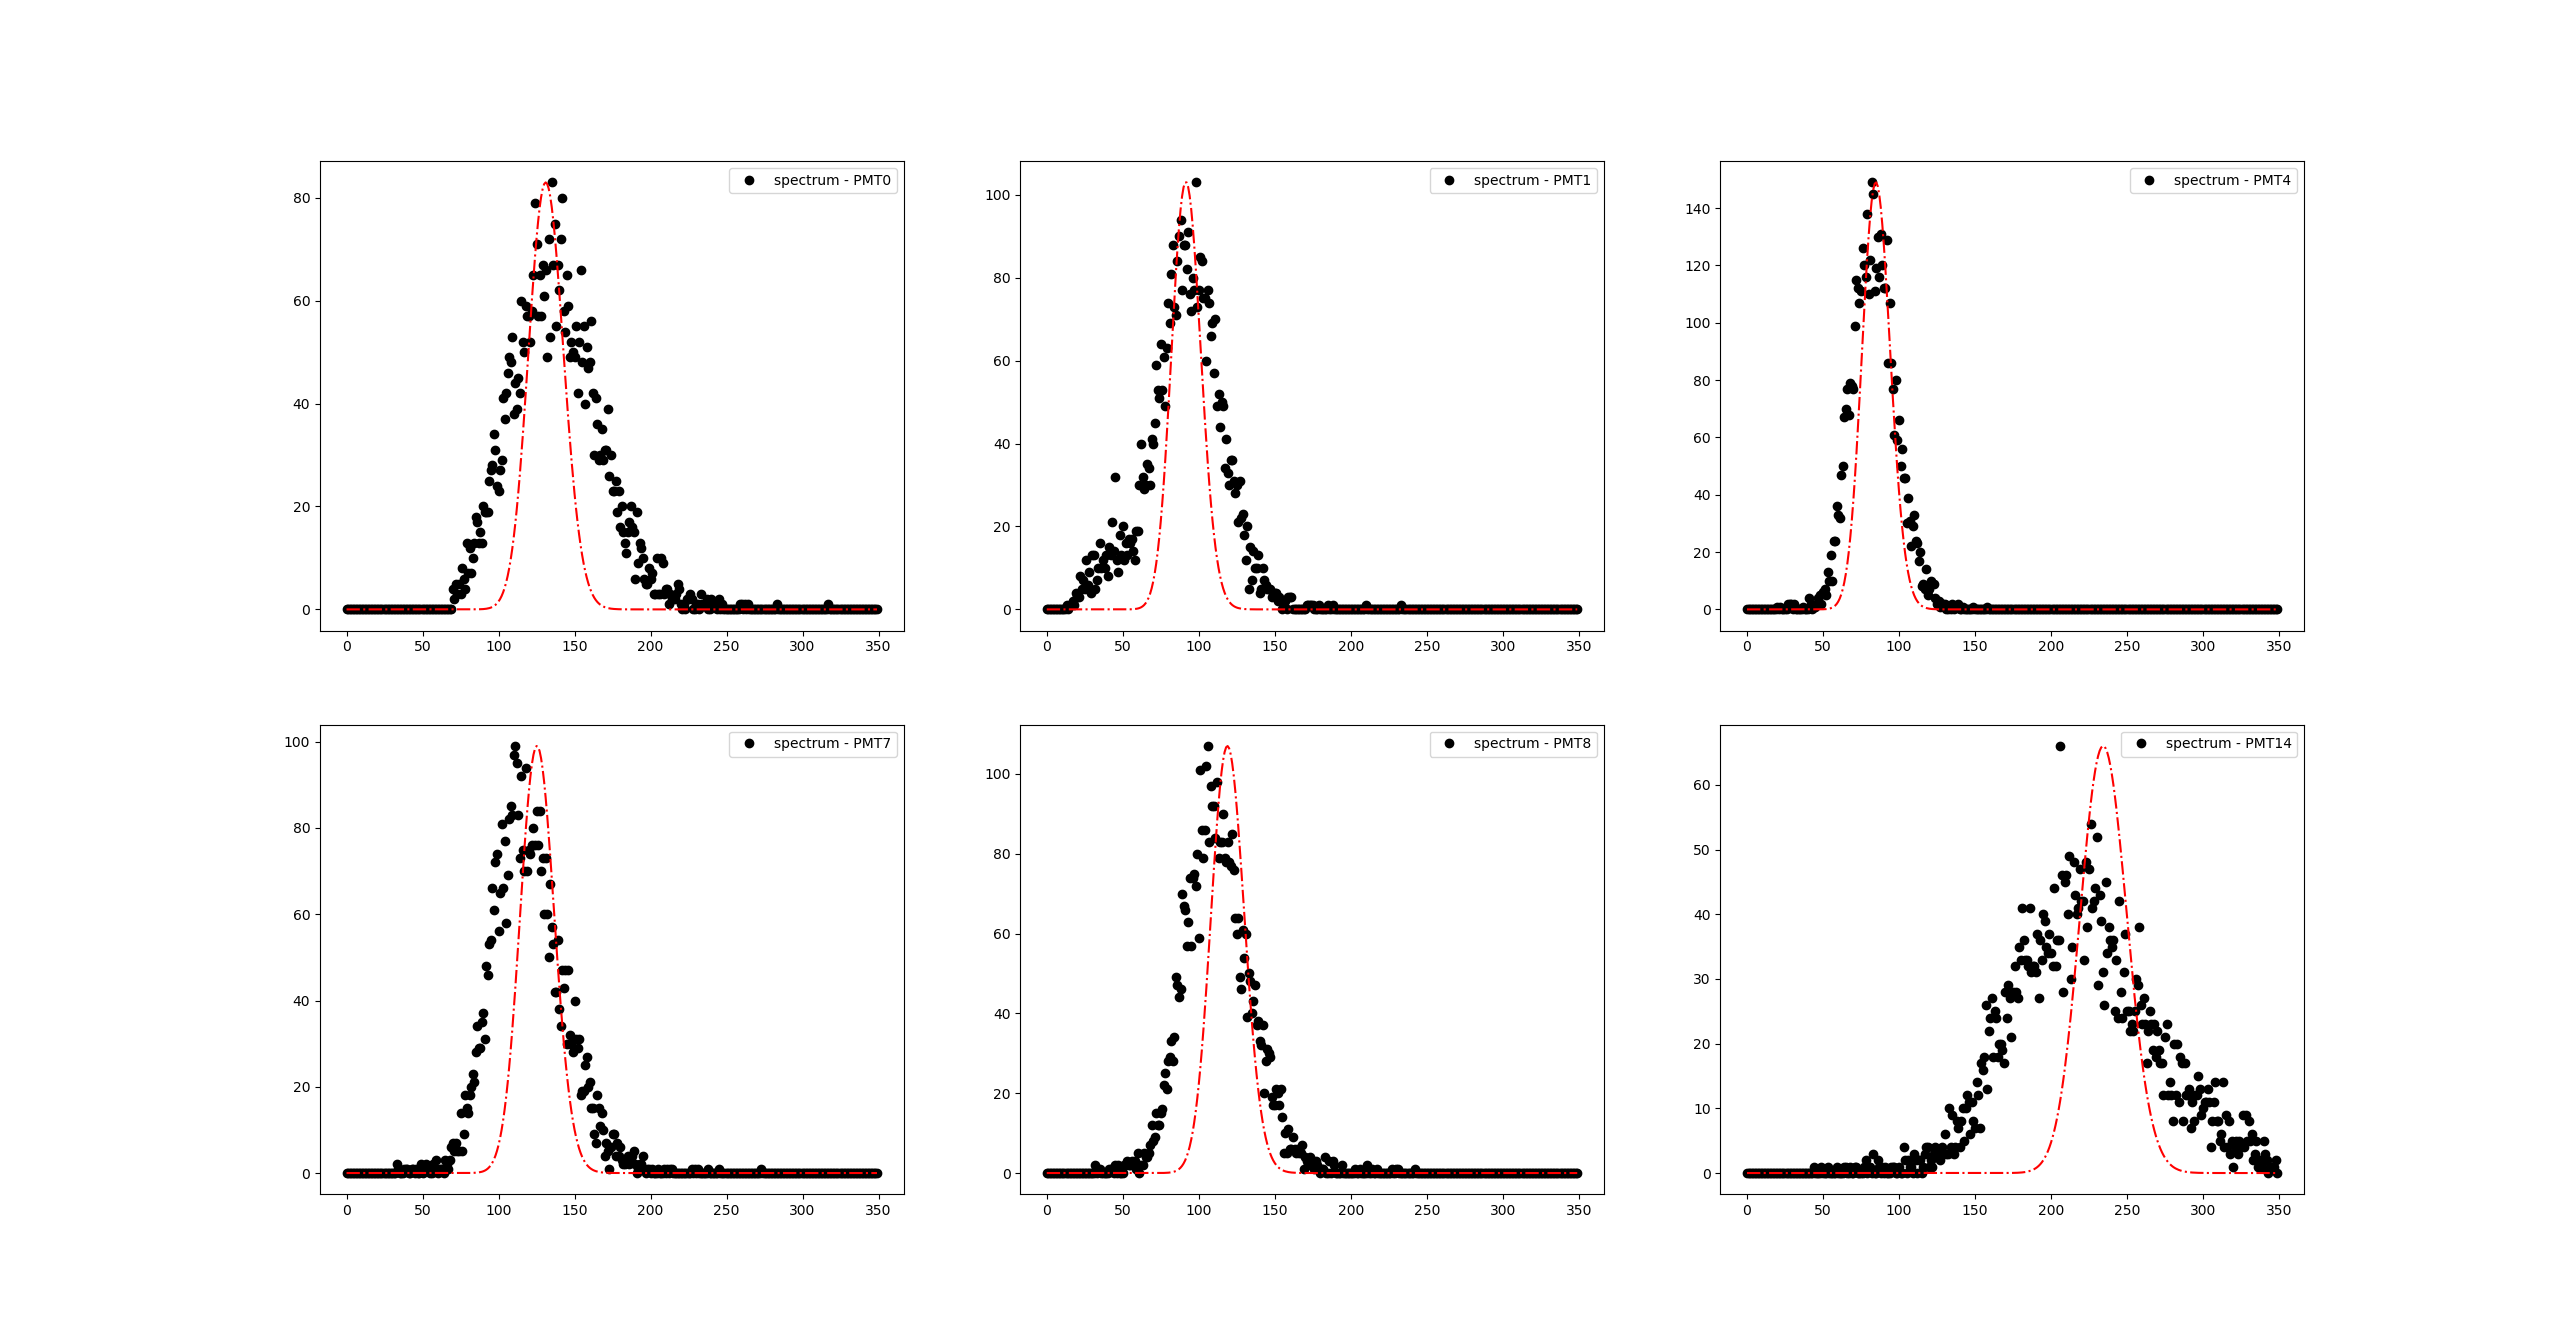
\includegraphics[width=1\textwidth]{Cs137Spec.png}
\end{figure}
\end{frame}

\begin{frame}{Fit - Temporal Uncertainty per PMT}
\begin{figure}[h]
\centering
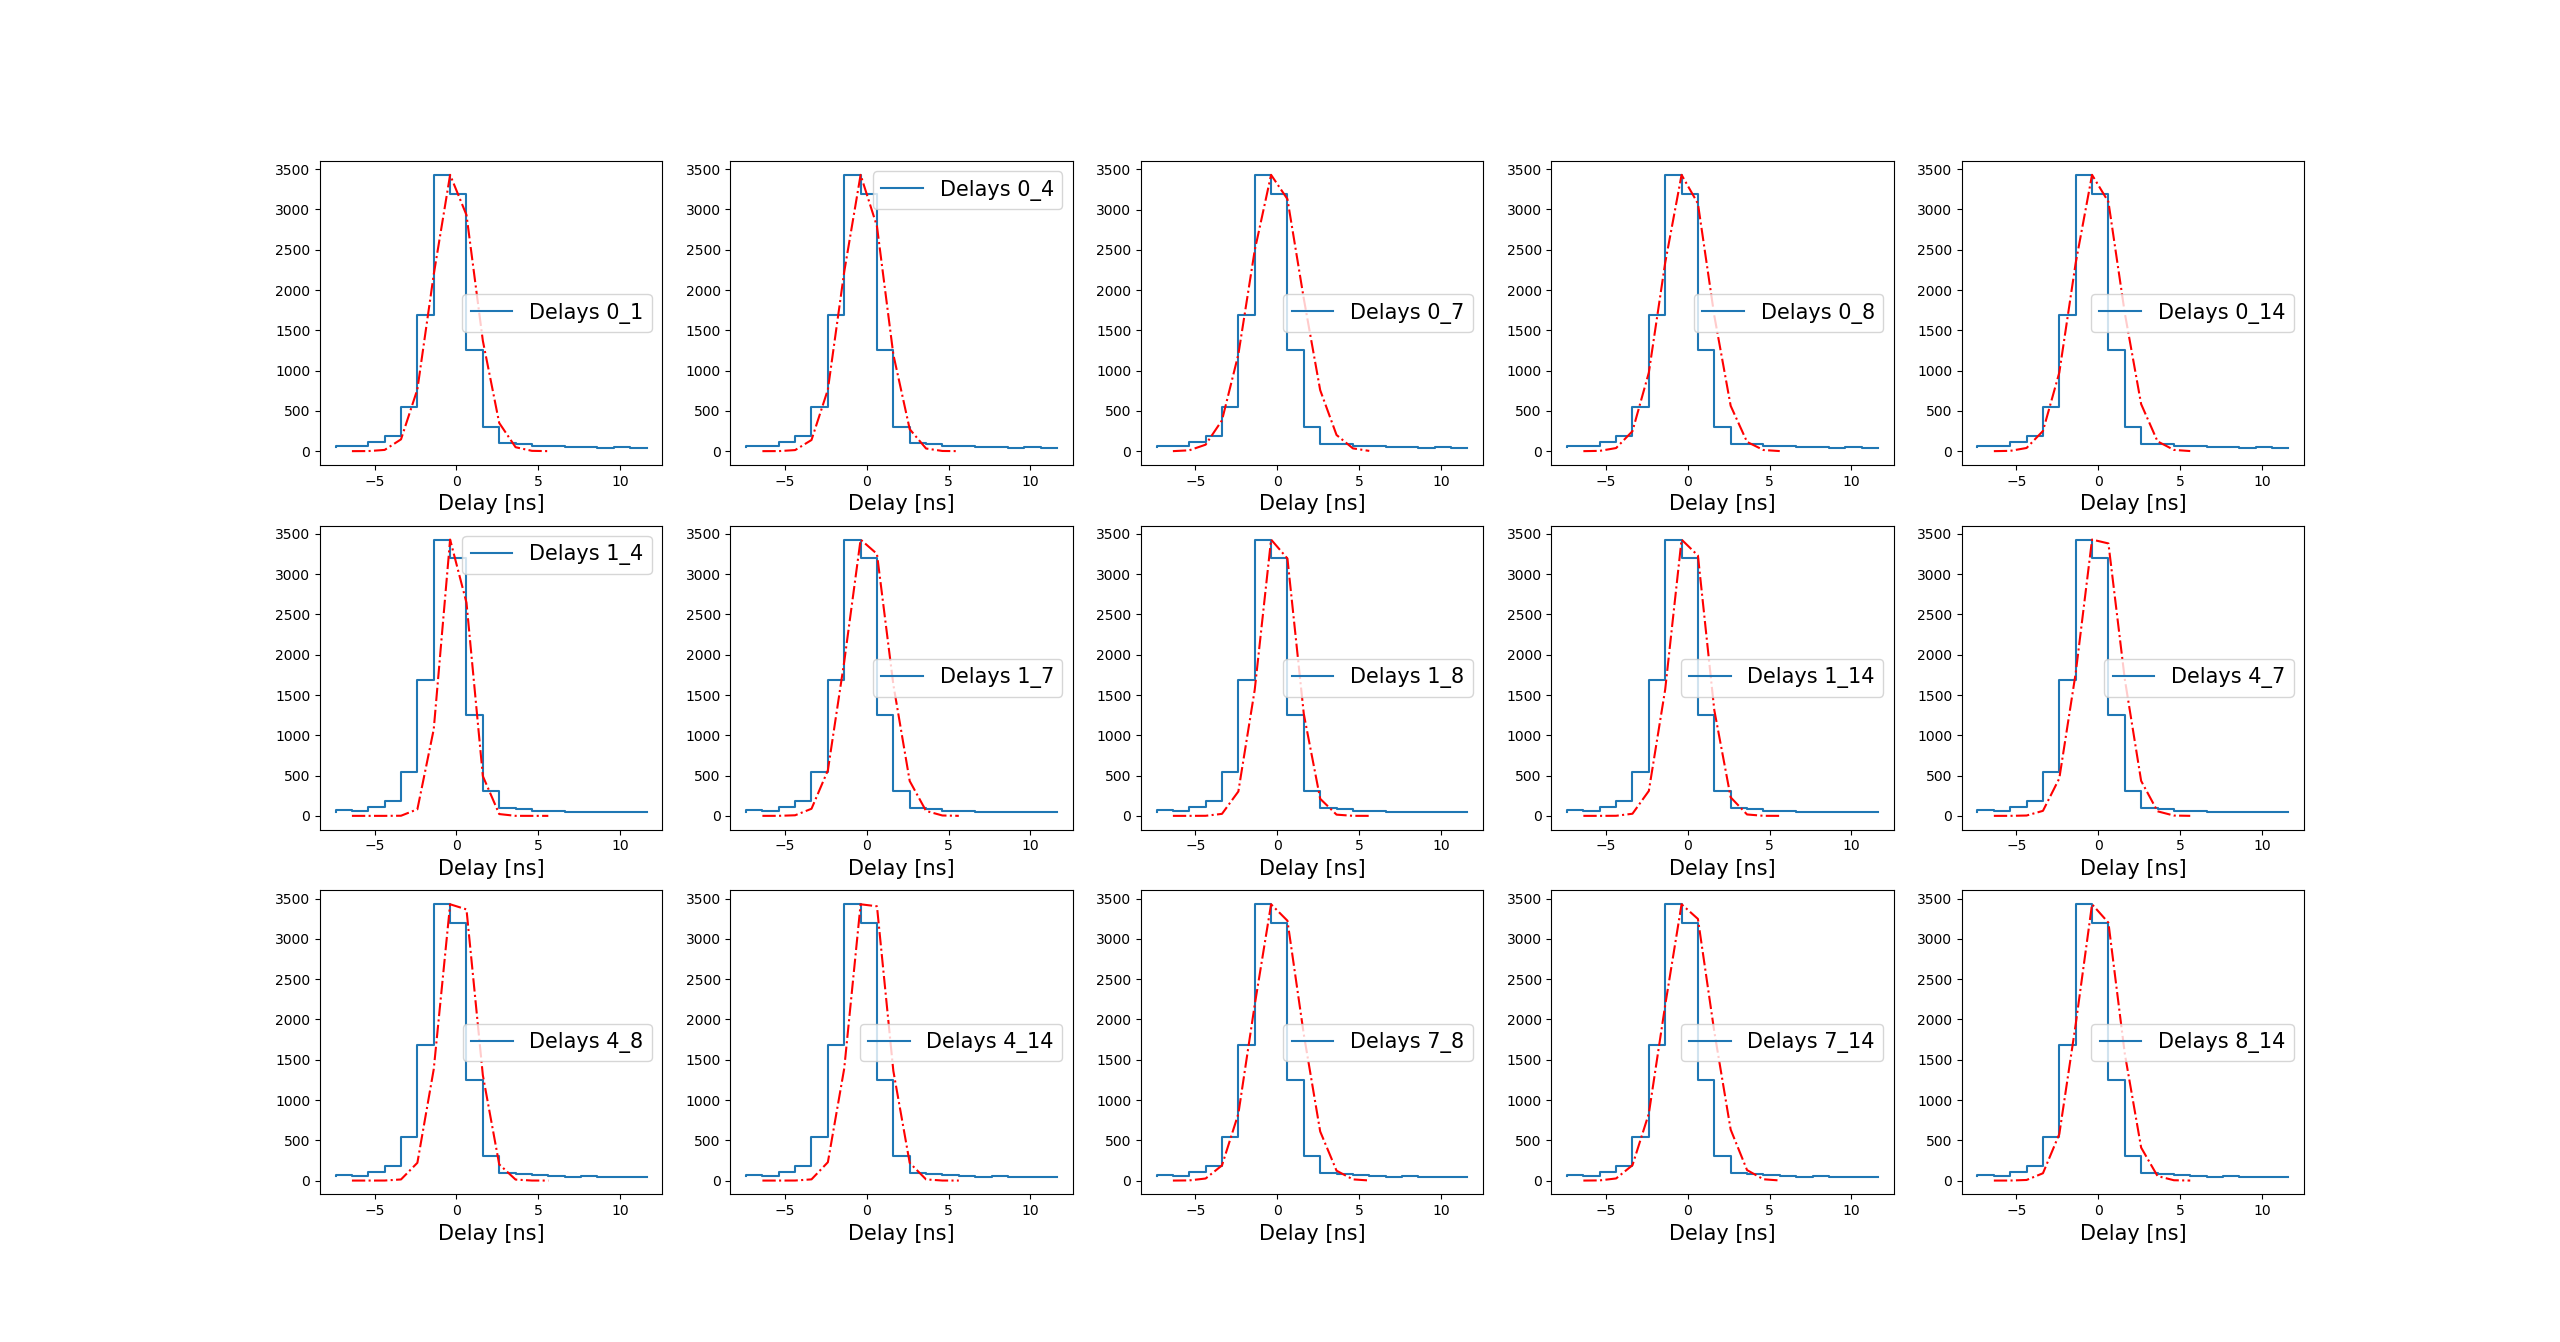
\includegraphics[width=1\textwidth]{Co57temp.png}
\end{figure}
\end{frame}

\begin{frame}{Fit - Temporal Distribution all PMTs - $^{57}$Co}
\begin{figure}[h]
\centering
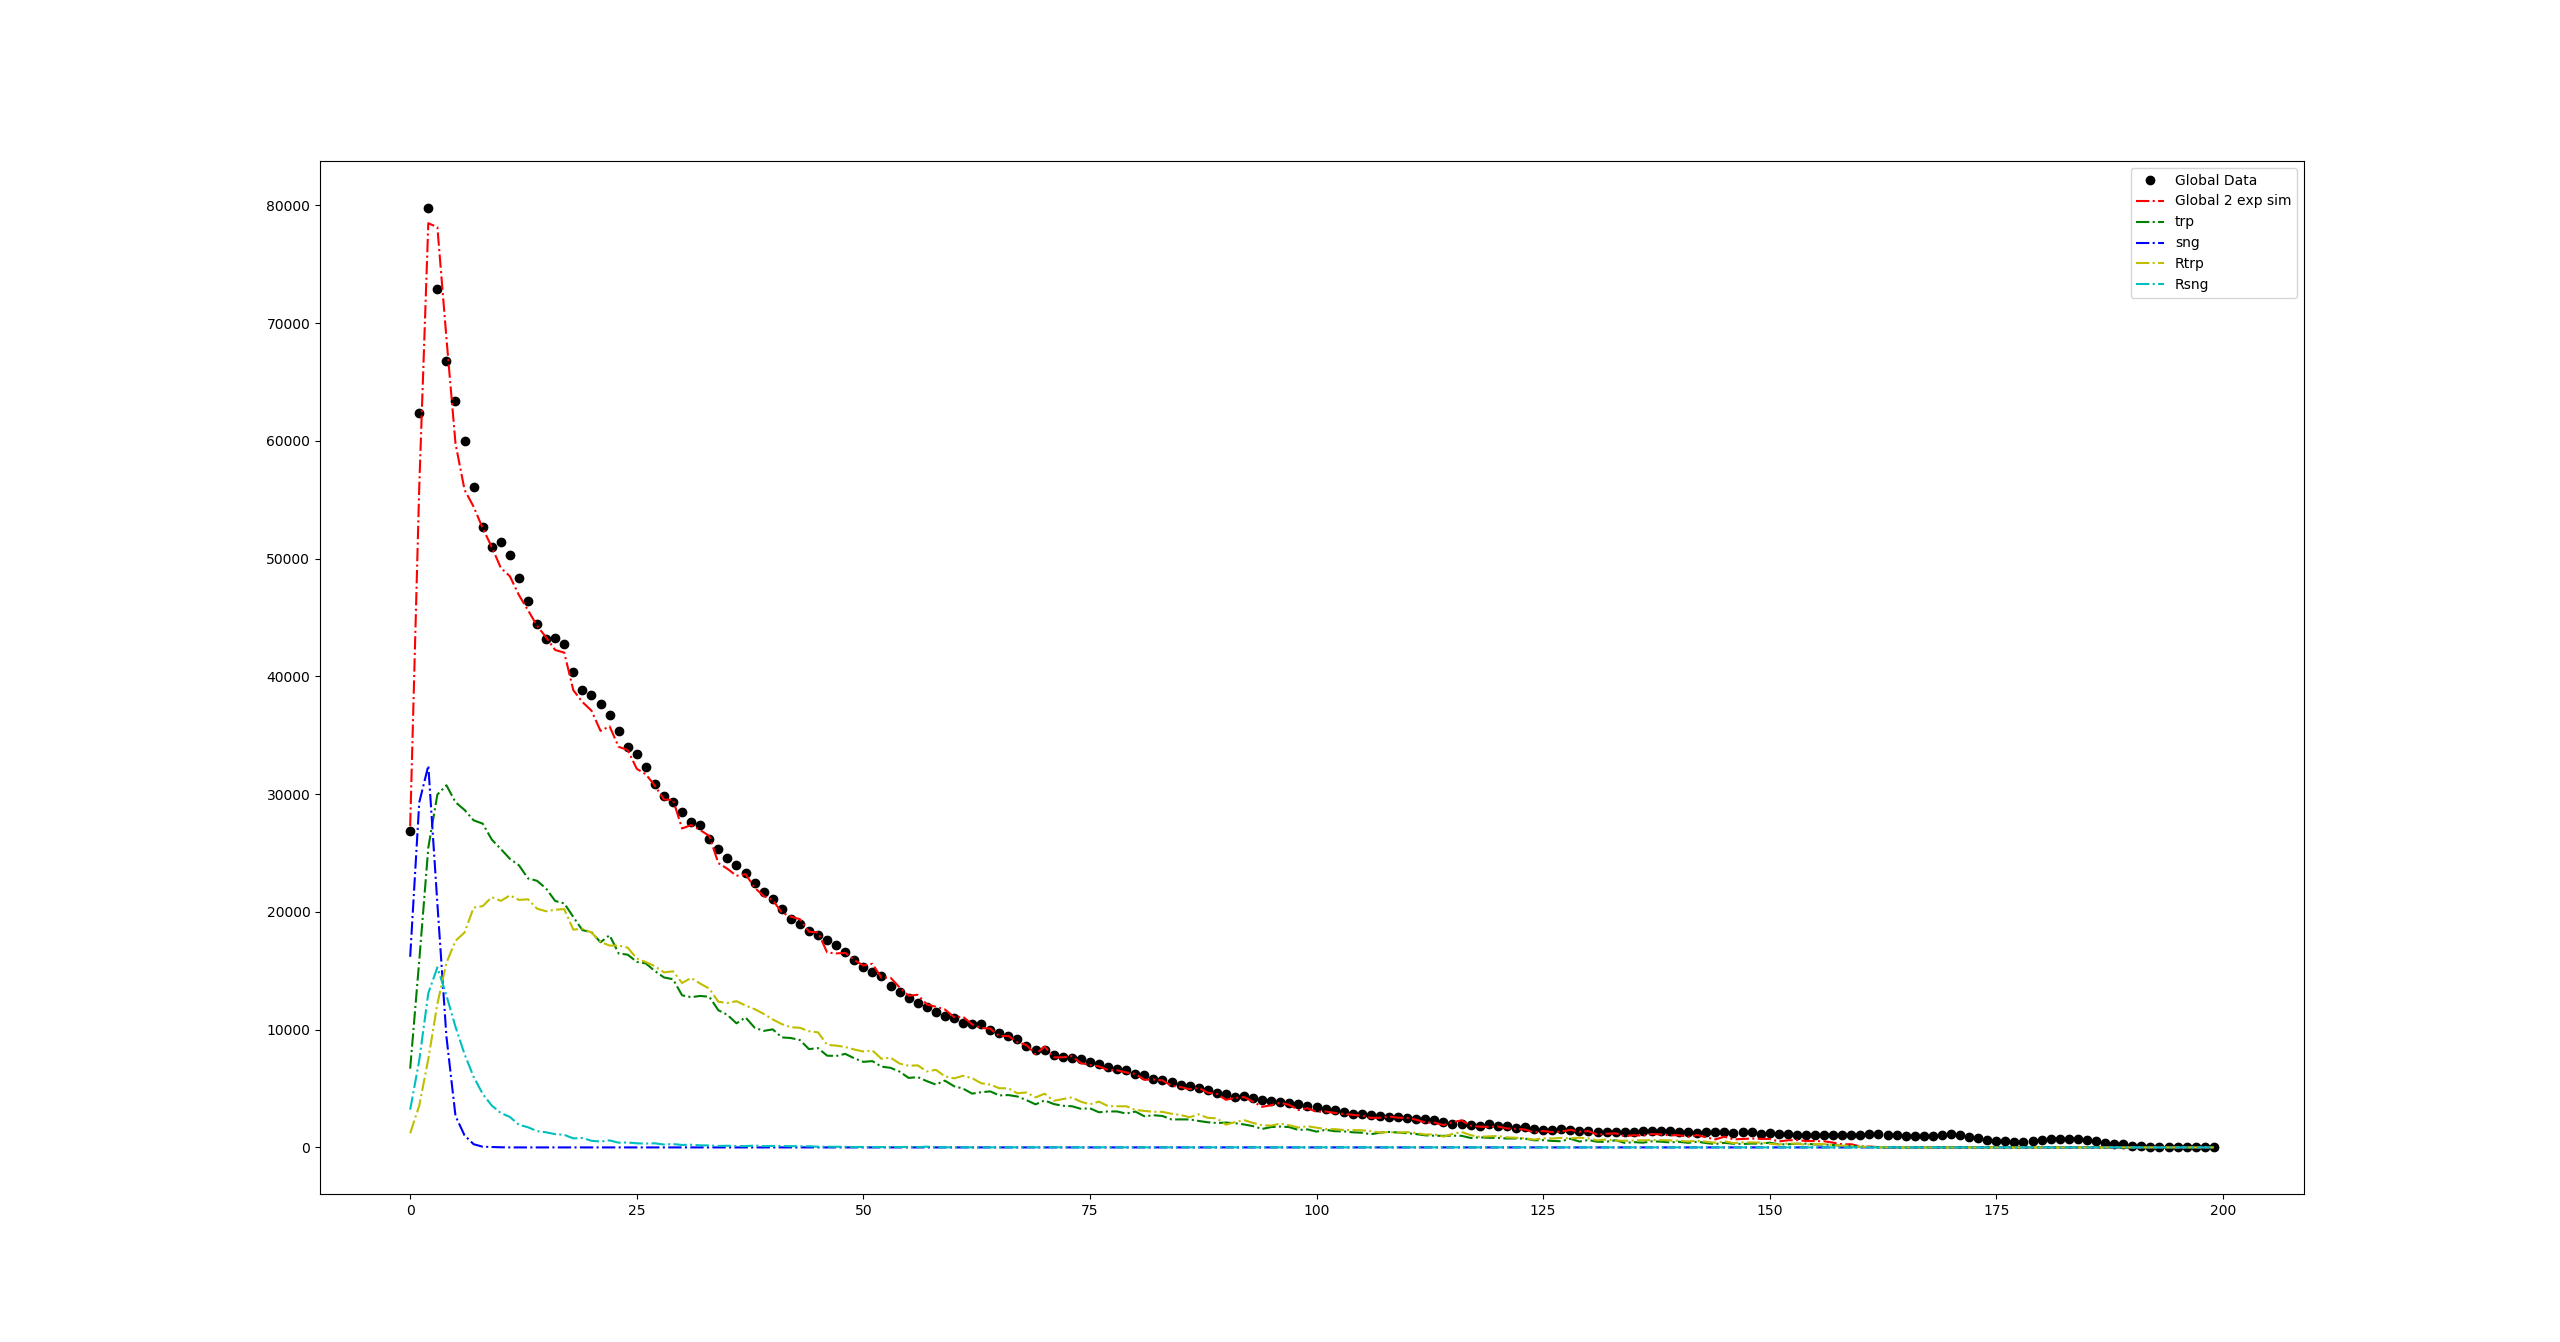
\includegraphics[width=1\textwidth]{Co57Glob.png}
\end{figure}
\end{frame}

\begin{frame}{Fit - Temporal Distribution all PMTs - $^{137}$Cs}
\begin{figure}[h]
\centering
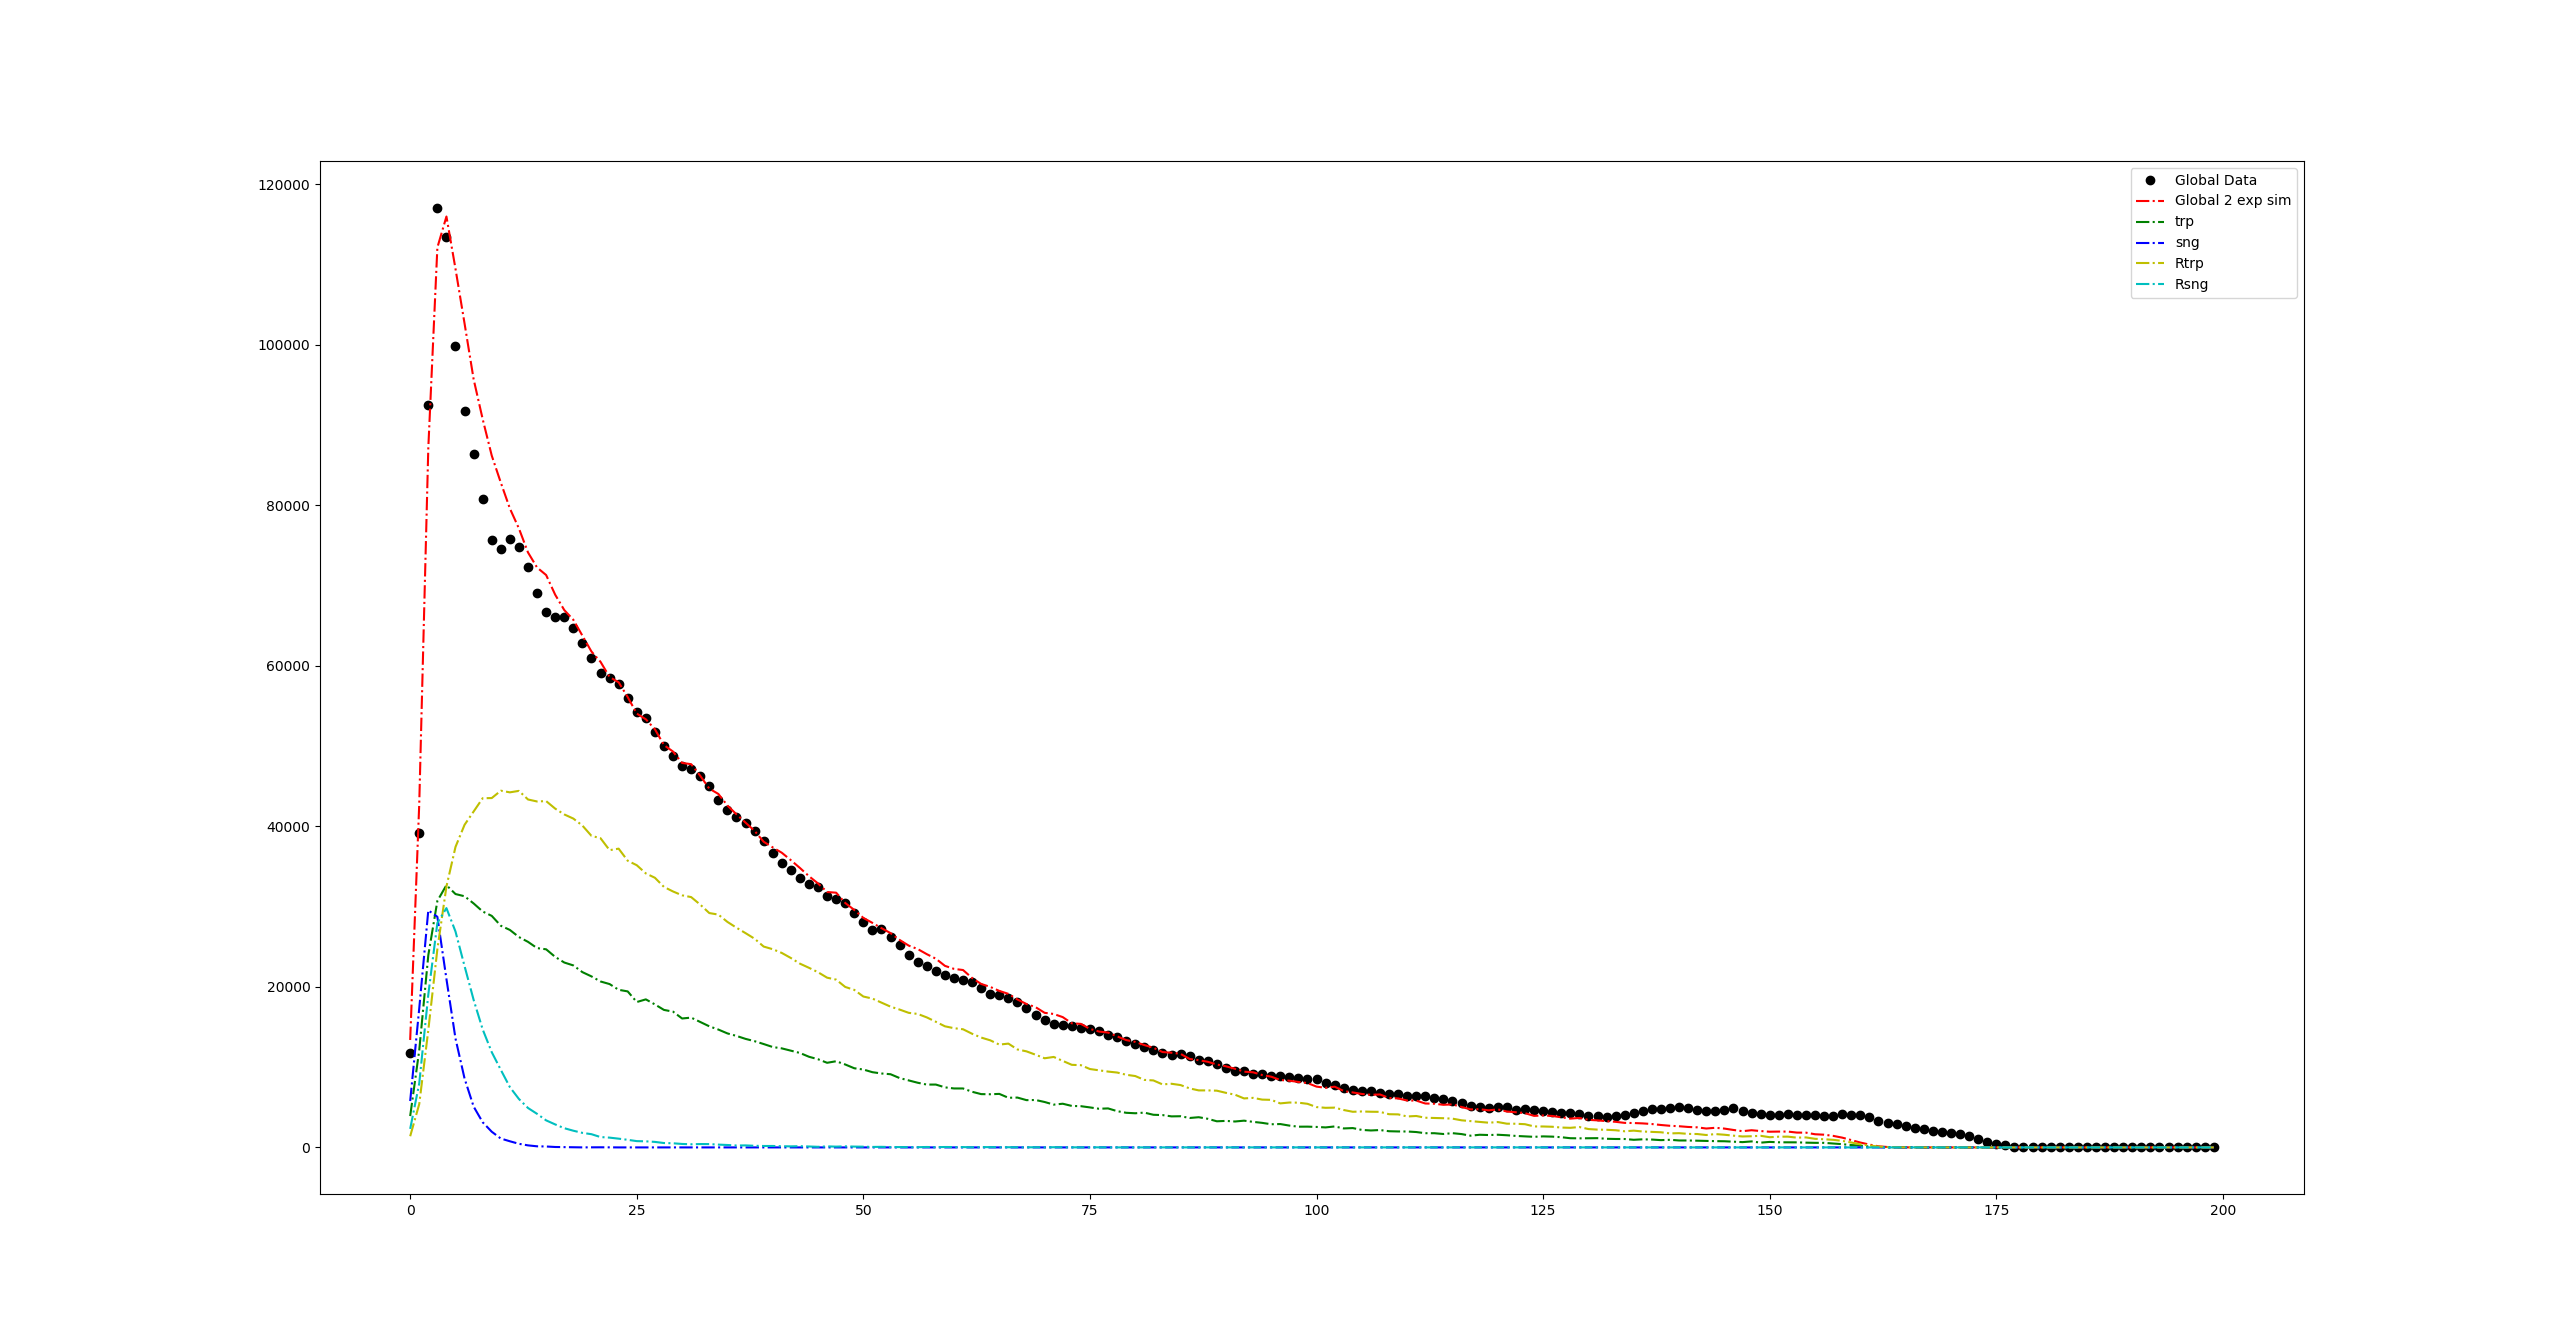
\includegraphics[width=1\textwidth]{CsGlob.png}
\end{figure}
\end{frame}

\begin{frame}{Primary Scintillation Parameters}
\begin{center}
\begin{tabular}{|c|c|c|c|}
\hline
&$F$ & $\tau_1$ [ns]& $\tau_3$ [ns]\\
\hline
Cs137 & 0.09 & 2 & 37 \\
\hline
Co57 & 0.09 & 0.8 & 31 \\
\hline
\end{tabular}
\end{center}
\begin{itemize}
\item $\tau_1$ should be $\sim2$ns.
\item $\tau_3$ is 22-27 ns (33 ns?). A better result may be achieved when we will fit the $\gamma$ sources simultaneously with the neutron source. 
\item $F$ is expected to increase with increase of the LET (energy decrees). If I understood it correctly there is a mechanism in which a singlet collides (superelasticly) with thermal electron and becomes triplet. For ERs this is suppressed because there Onsager recombination factor is constant in energy but for NRs it is much higher so there are less thermal electrons.
\end{itemize}
\end{frame}

\begin{frame}{Recombination Parameters}
\begin{center}
\begin{tabular}{|c|c|c|c|}
\hline
&$R$ & $\alpha$ [ns]$^{-1}$& $\eta$\\
\hline
Cs137 & 0.68 & 0.45 & 0.2 \\
\hline
Co57 & 0.54 & 0.35 & 0.2 \\
\hline
\end{tabular}
\end{center}
\begin{itemize}
\item $R$ isn't energy dependent. The branching between the excitation and ionization is measured to be 0.06.
\begin{equation}
\frac{I_{ex}}{I_{ion}}=\frac{1-R-C}{R+C}
\end{equation}
$C=0.57$ (from NEST).
\end{itemize}
\end{frame}

\end{document}

